\documentclass{beamer}
\mode<presentation>
{
\usetheme{Boadilla}
%\setbeamercovered{transparent}
\usecolortheme{whale}
}
\setbeamertemplate{footline}[frame number]


\newcommand{\independent}{\perp\!\!\!\!\perp} 
\usepackage{bibentry}
\nobibliography*
\usepackage{pdfpages}
\usepackage{graphicx}
\usepackage{pgf}
\usepackage{hyperref}
\usepackage{amsmath,amsfonts,nicefrac,amssymb}
\usepackage{graphicx}
%\usepackage{enumerate}
\usepackage{multicol}
\usepackage[square,sort,colon]{natbib}
\usepackage{pdfpages}
\usepackage{url}
\usepackage{ifthen}
\usepackage{subcaption}
\usepackage{longtable}
\usepackage{pdfpages}
\usetheme{Boadilla}
\usepackage{tikz}
\usepackage{environ}
\usepackage{lipsum}
\usepackage{booktabs}
\usepackage{xcolor,colortbl}
%\usepackage{enumitem}
\beamertemplatefootpagenumber


%\newenvironment{slide}[1]
%{\begin{frame}[environment=slide]
%\frametitle{\insertsection}}
%{\end{frame}}
%\setbeamertemplate{caption}[numbered]
\setcounter{page}{1}

\title[]{A Structured Framework for Adaptively Incorporating External Evidence in Sequentially Monitored Clinical Trials} 
\author[]{Evan Kwiatkowski\textsuperscript{1}, Eugenio Andraca-Carrera\textsuperscript{2}, Mat Soukup\textsuperscript{2}, Matthew A. Psioda\textsuperscript{1}}
%{ \normalsize{		
%			Evan Kwiatkowski\textsuperscript{1}, Eugenio Andraca-Carrera\textsuperscript{2}, 
%			Mat Soukup\textsuperscript{2}, Matthew A. Psioda\textsuperscript{1}\\
%
%
%			\textsuperscript{1} Department of Biostatistics, University of \\
%			North Carolina, McGavran-Greenberg Hall, CB\#7420 \\
%
%
%			\textsuperscript{2}{Division of Biometrics VII, Office of Biostatistics, Center for Drug Evaluation and Research, US Food and Drug Administration, Silver Spring, Maryland, USA}}}
\institute{
\textsuperscript{1} Department of Biostatistics, University of North Carolina at Chapel Hill\\
\textsuperscript{2}Division of Biometrics VII, Office of Biostatistics, Center for Drug Evaluation and Research, US Food and Drug Administration
}
\date{\scriptsize{August 12$\textsuperscript{th}$, 2021}}

\begin{document}
\beamertemplatefootpagenumber
\maketitle

%\begin{frame}{Motivation}
%\begin{itemize}
%\item We present a structured framework for specifying monitoring priors and stoppage criteria for a Bayesian sequentially monitored clinical trial that is based on intuitive justification for the design quantities rather than being motivated by having pre-specified frequentist operating characteristics.
%\end{itemize}
%\end{frame}


%\begin{frame}{Enthusiastic Monitoring Prior}
%\begin{itemize}
%\item Consider again the hypotheses $H_0: \theta \le \theta_0$ versus $H_1: \theta > \theta_0$ where $\theta_0$ represents a 
%treatment effect of interest and let $\theta_1>\theta_0$ represent a plausible, clinically meaningful effect.
%%
%\item Define an enthusiastic prior, denoted as $\pi_{E}(\theta)$, as a prior consistent with $\theta_1$ being the most 
%likely value of $\theta$ (i.e., the prior mode) and that reflects the belief of an observer who is 
%\textit{all but convinced} that $H_1$ is true a priori. 
%%
%\item Formally, this is defined as satisfying (i) $\text{argmax}_\theta~\pi_E(\theta)=\theta_1$
%and (ii) $P_E(\theta >\theta_0)=1-\epsilon$, where the subscript $E$ indicates that the probability is 
%based on $\pi_{E}(\theta)$.
%\end{itemize}
%\end{frame}
%
%\begin{frame}{Skeptical Monitoring Prior}
%\begin{itemize}
%\item 
%Similarly, define a skeptical prior, denoted as $\pi_{S}(\theta)$, as a prior consistent with $\theta_0$ being the most 
%likely value of $\theta$ and that reflects the belief of an observer who is \textit{all but convinced} that 
%$\theta <\theta_1$ is true a priori. 
%%
%\item Formally, this is defined as the prior $\pi_{S}(\theta)$ satisfying
%(iii) $\text{argmax}_\theta~\pi_S(\theta)=\theta_0$  and (iv) $P_S(\theta <\theta_1)=1-\epsilon$.
%%
%In what follows we refer to (i) and (iii) as \textit{mode value constraints} and (ii) and (iv) as \textit{tail-probability constraints}, respectively.
%\end{itemize}
%\end{frame}

%\begin{frame}{Generalized Normal Distribution}
%\begin{itemize}
%\item 
%The density for a generalized normal distribution $\mathcal{GN}(\mu,\alpha,\beta)$ is
%\begin{align*}
%f(\theta)=\frac{\beta}{2\alpha\Gamma(1/\beta)}\exp\left\{-\left(\frac{|\theta-\mu|}{\alpha}\right)^\beta\right\}
%\end{align*} where $\mu$ is a location parameter, $\alpha>0$ is a scale parameter, and $\beta>0$ is a shape parameter. 
%\item
%A monitoring prior in the generalized normal family of distributions can have density at the mode equal to $k\times \frac{1}{\sqrt{2\pi}\sigma}$, with $k<1$ indicating a more flattened distribution and $k>1$ indicating a more peaked distribution at the mode, relative to the default normal distribution. 
%\end{itemize}
%\end{frame}

\begin{frame}{Skeptical Monitoring Prior}
\begin{figure}[htbp]
\begin{center}
%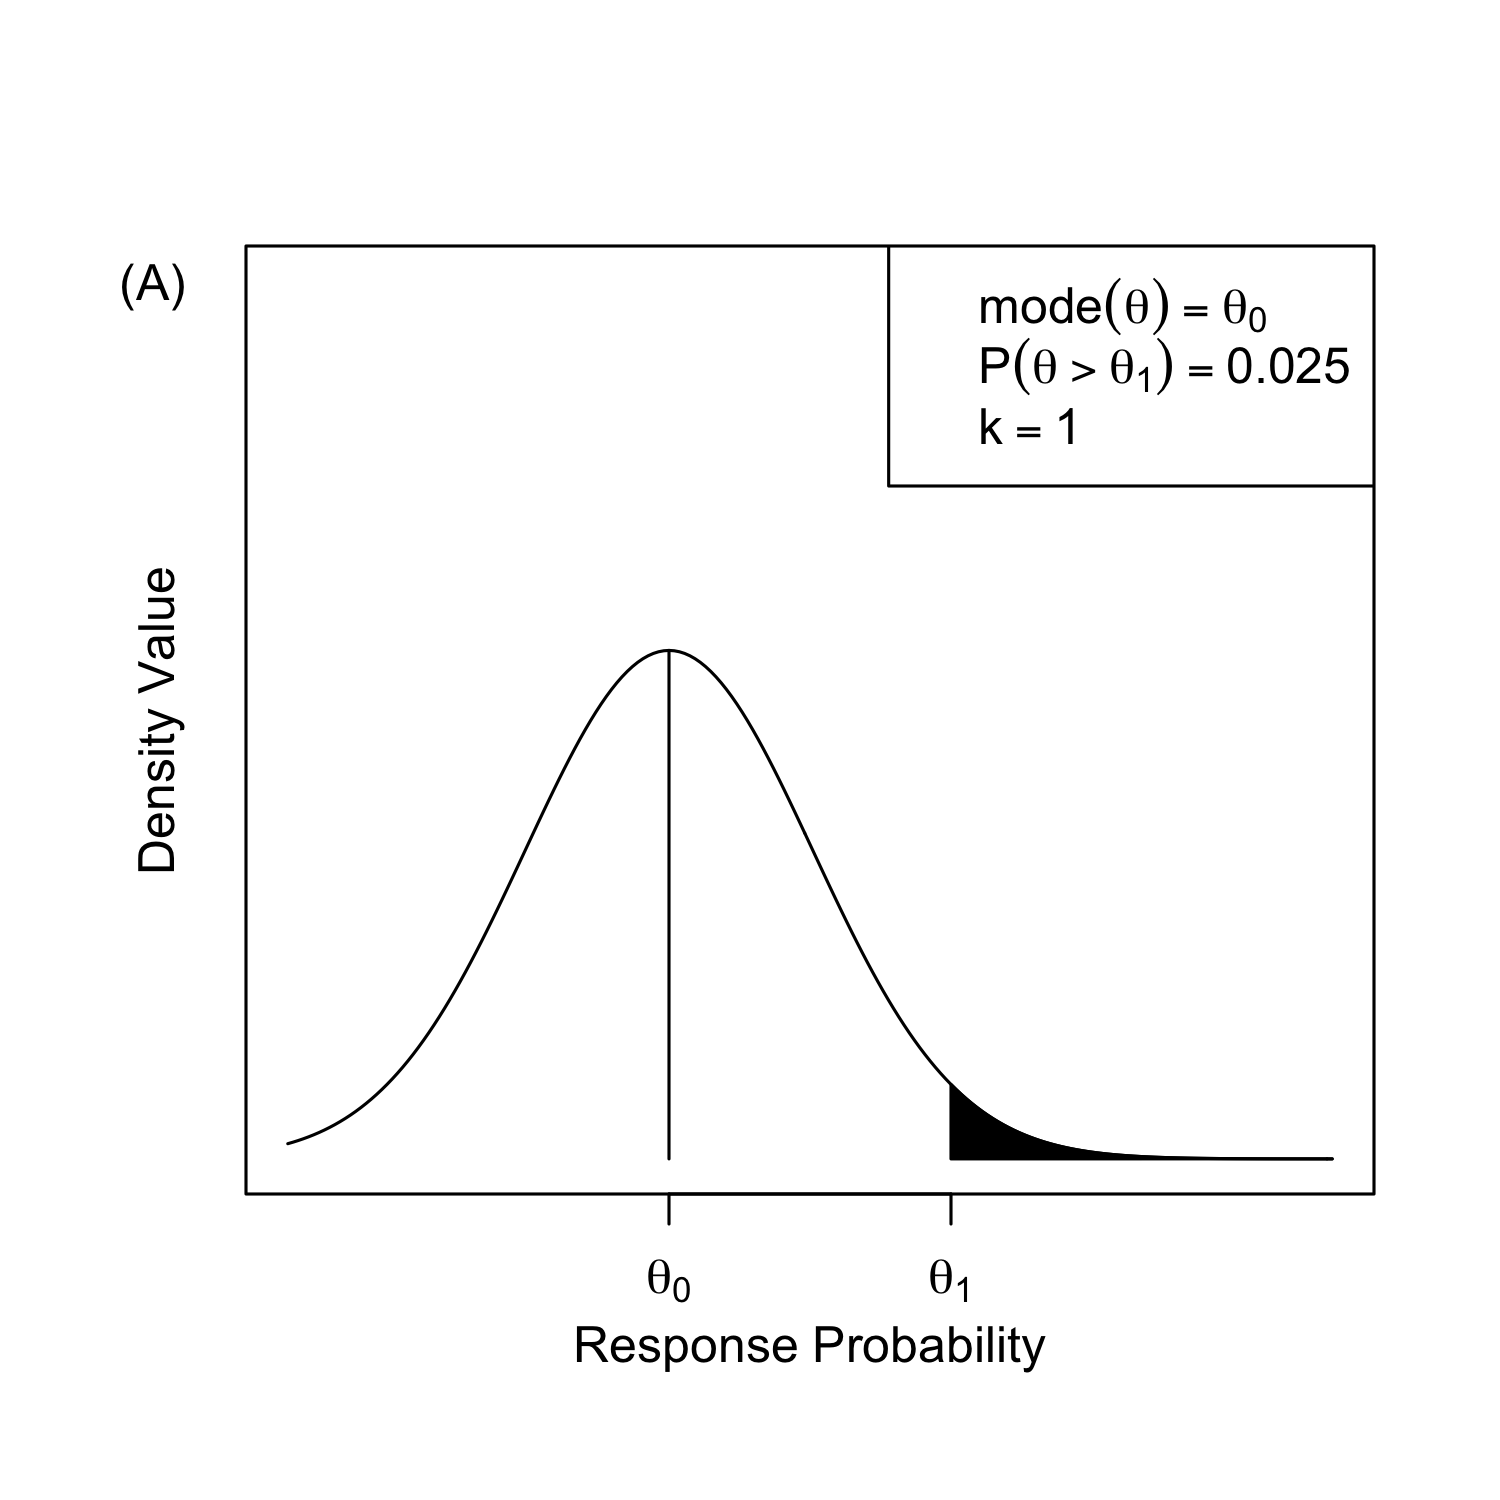
\includegraphics[width=2in]{./figures/figure1a.png}
%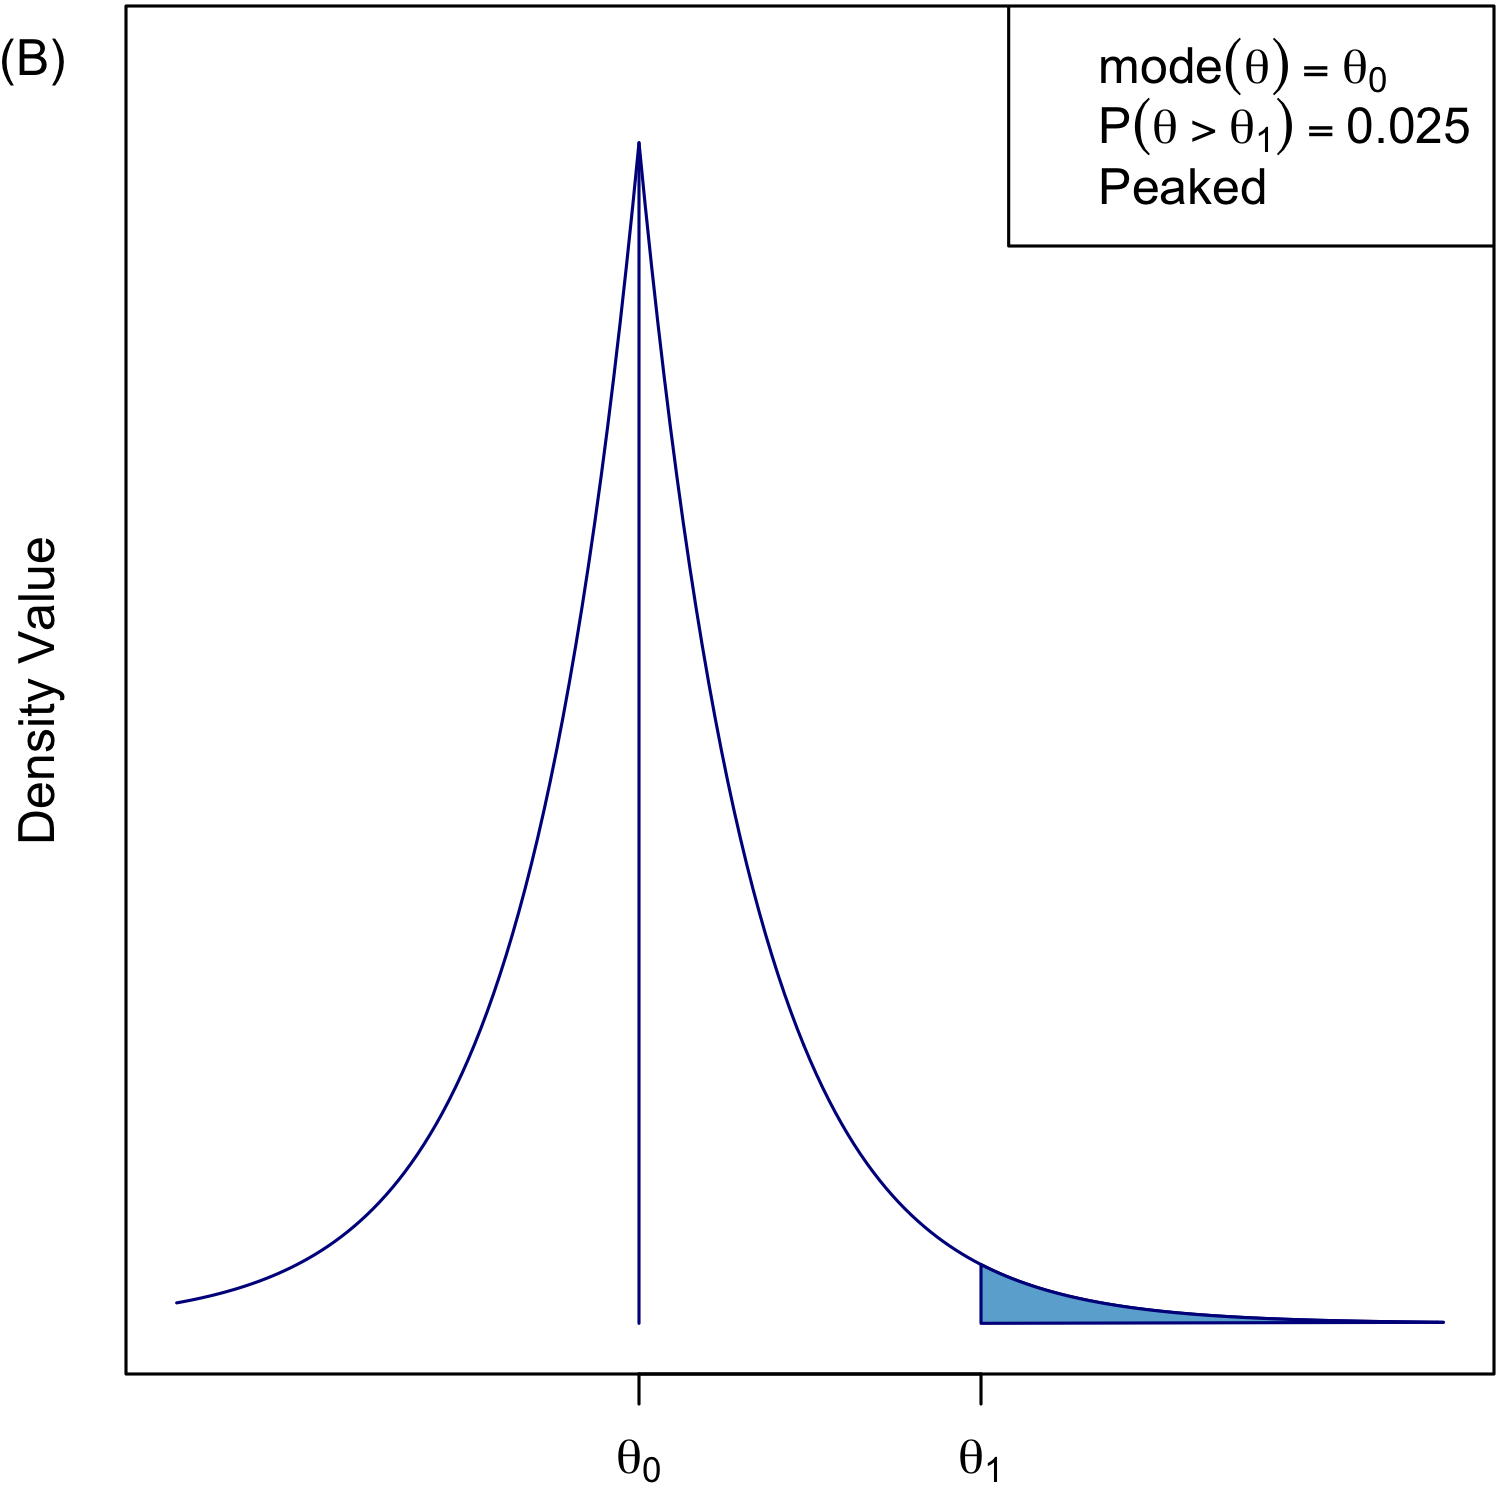
\includegraphics[width=2in]{./figures/figure1b.png}
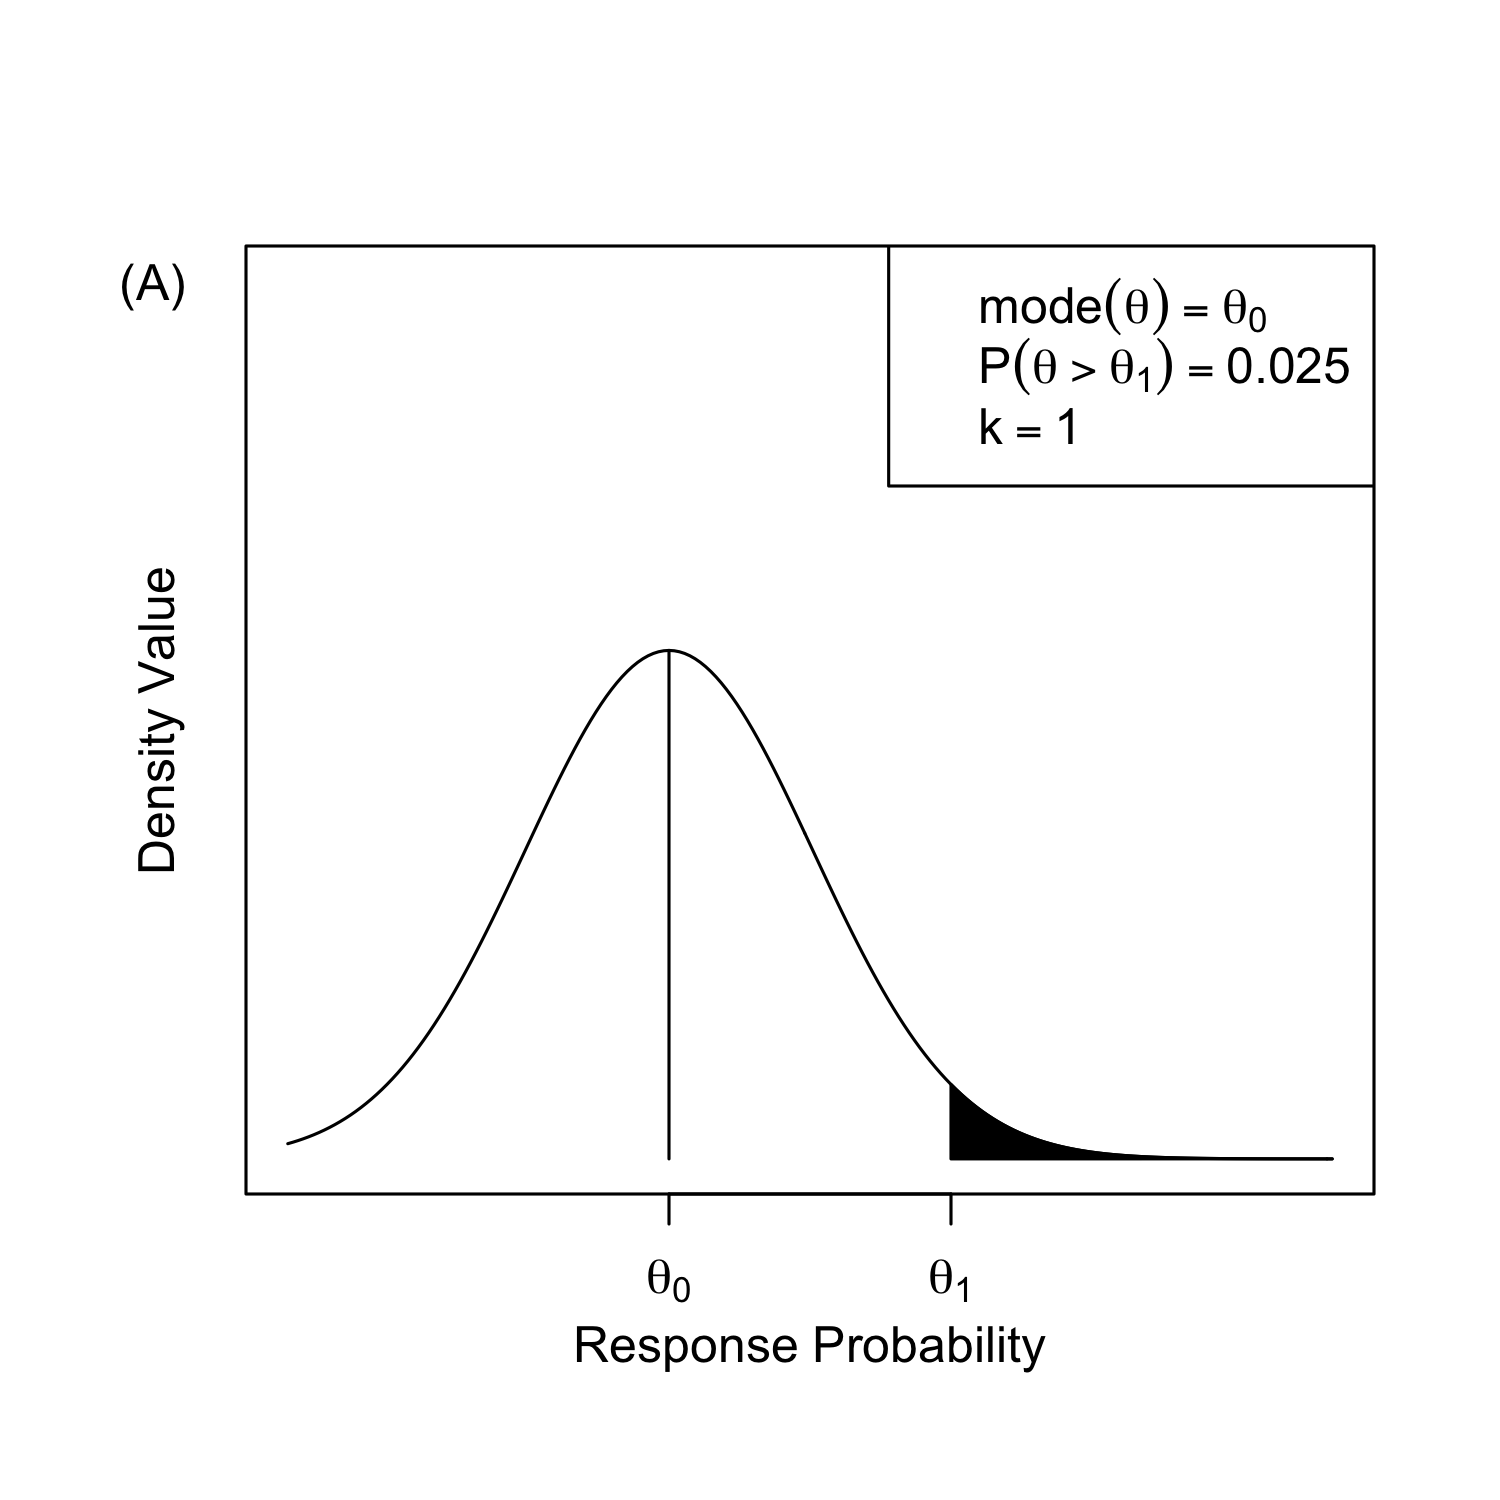
\includegraphics[width=0.5\textwidth]{./figures/figure1a.png}%
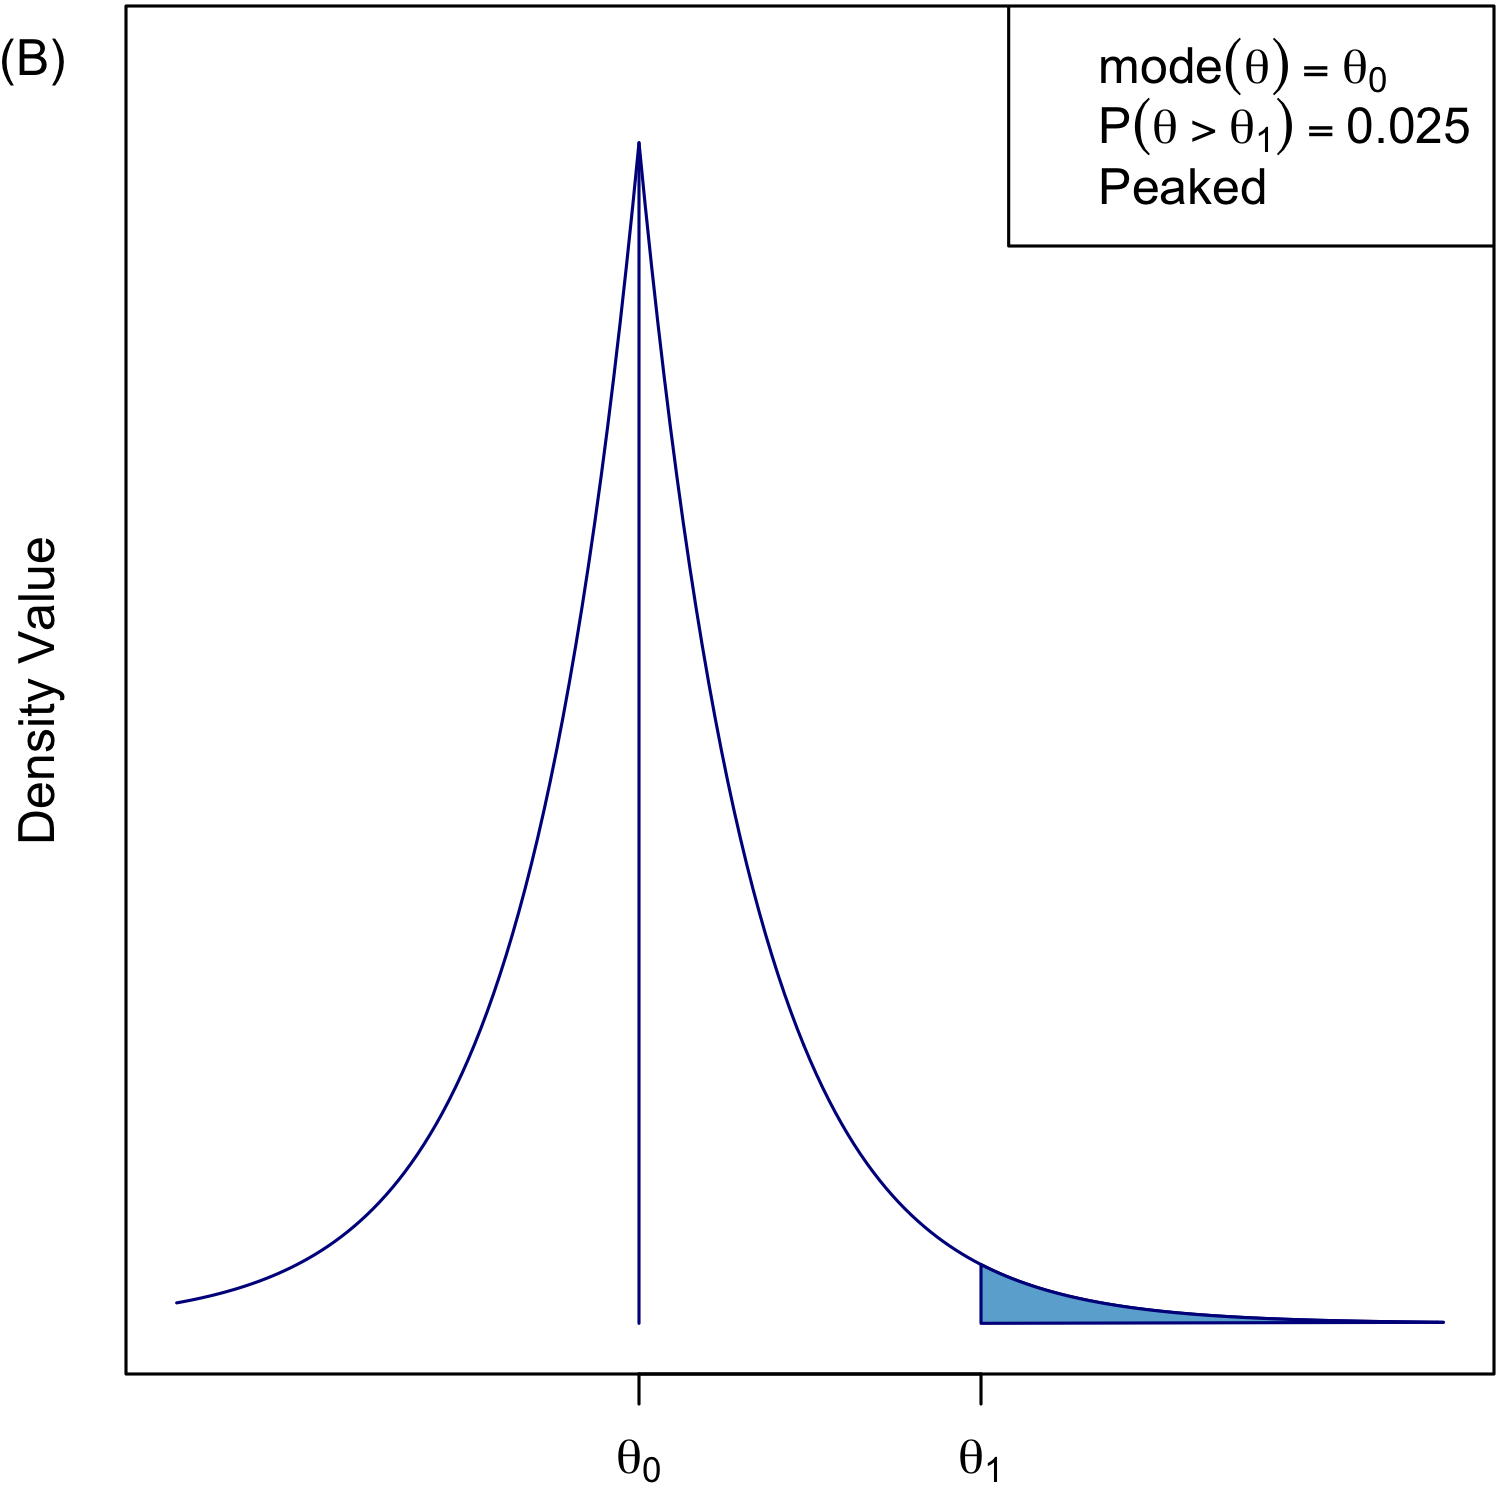
\includegraphics[width=0.5\textwidth]{./figures/figure1b.png}
\caption{A, Default skeptical prior. B, Concentrated skeptical prior.}

\label{fig:figure1}
\end{center}
\end{figure}
\end{frame}

\begin{frame}{Enthusiastic Monitoring Prior}
\begin{figure}[htbp]
\begin{center}
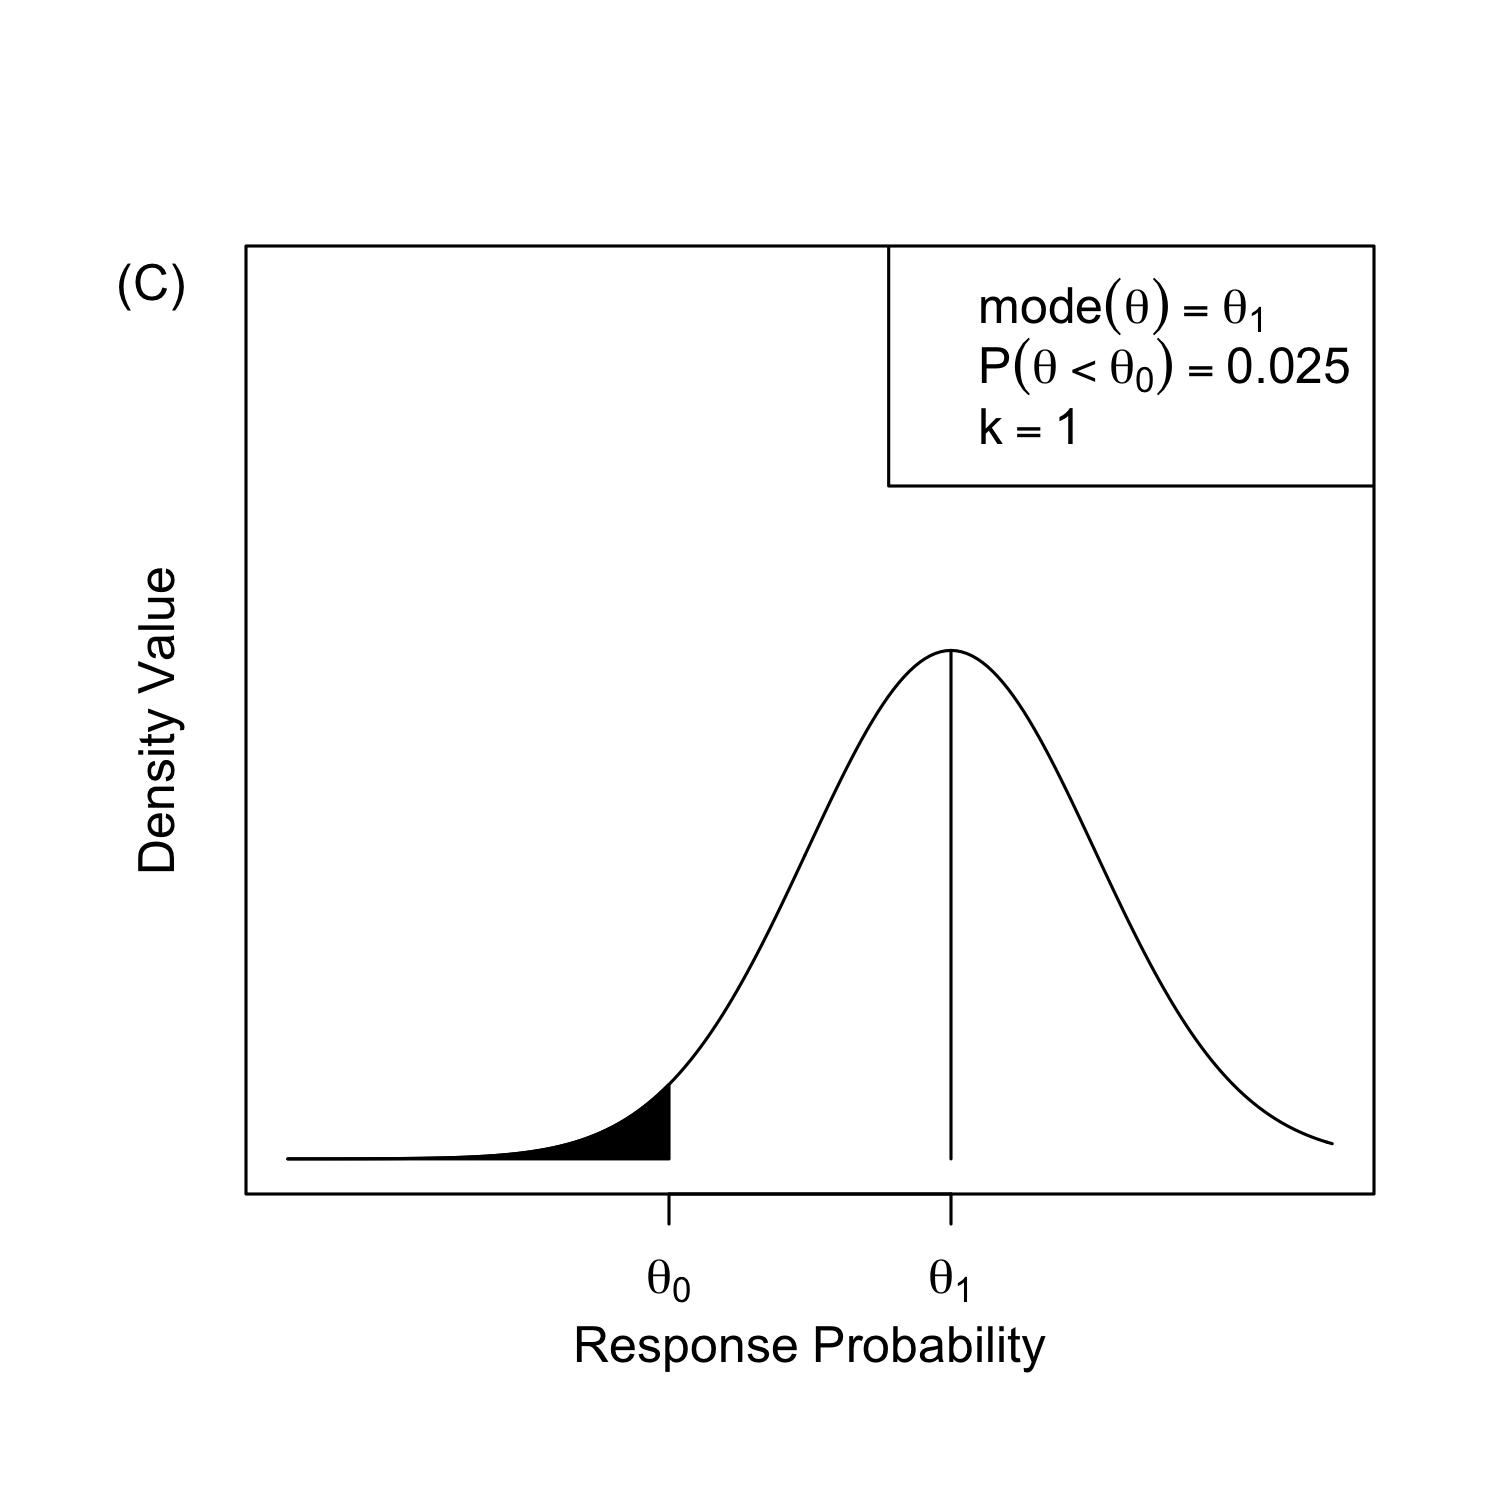
\includegraphics[width=0.5\textwidth]{./figures/figure1c.png}%
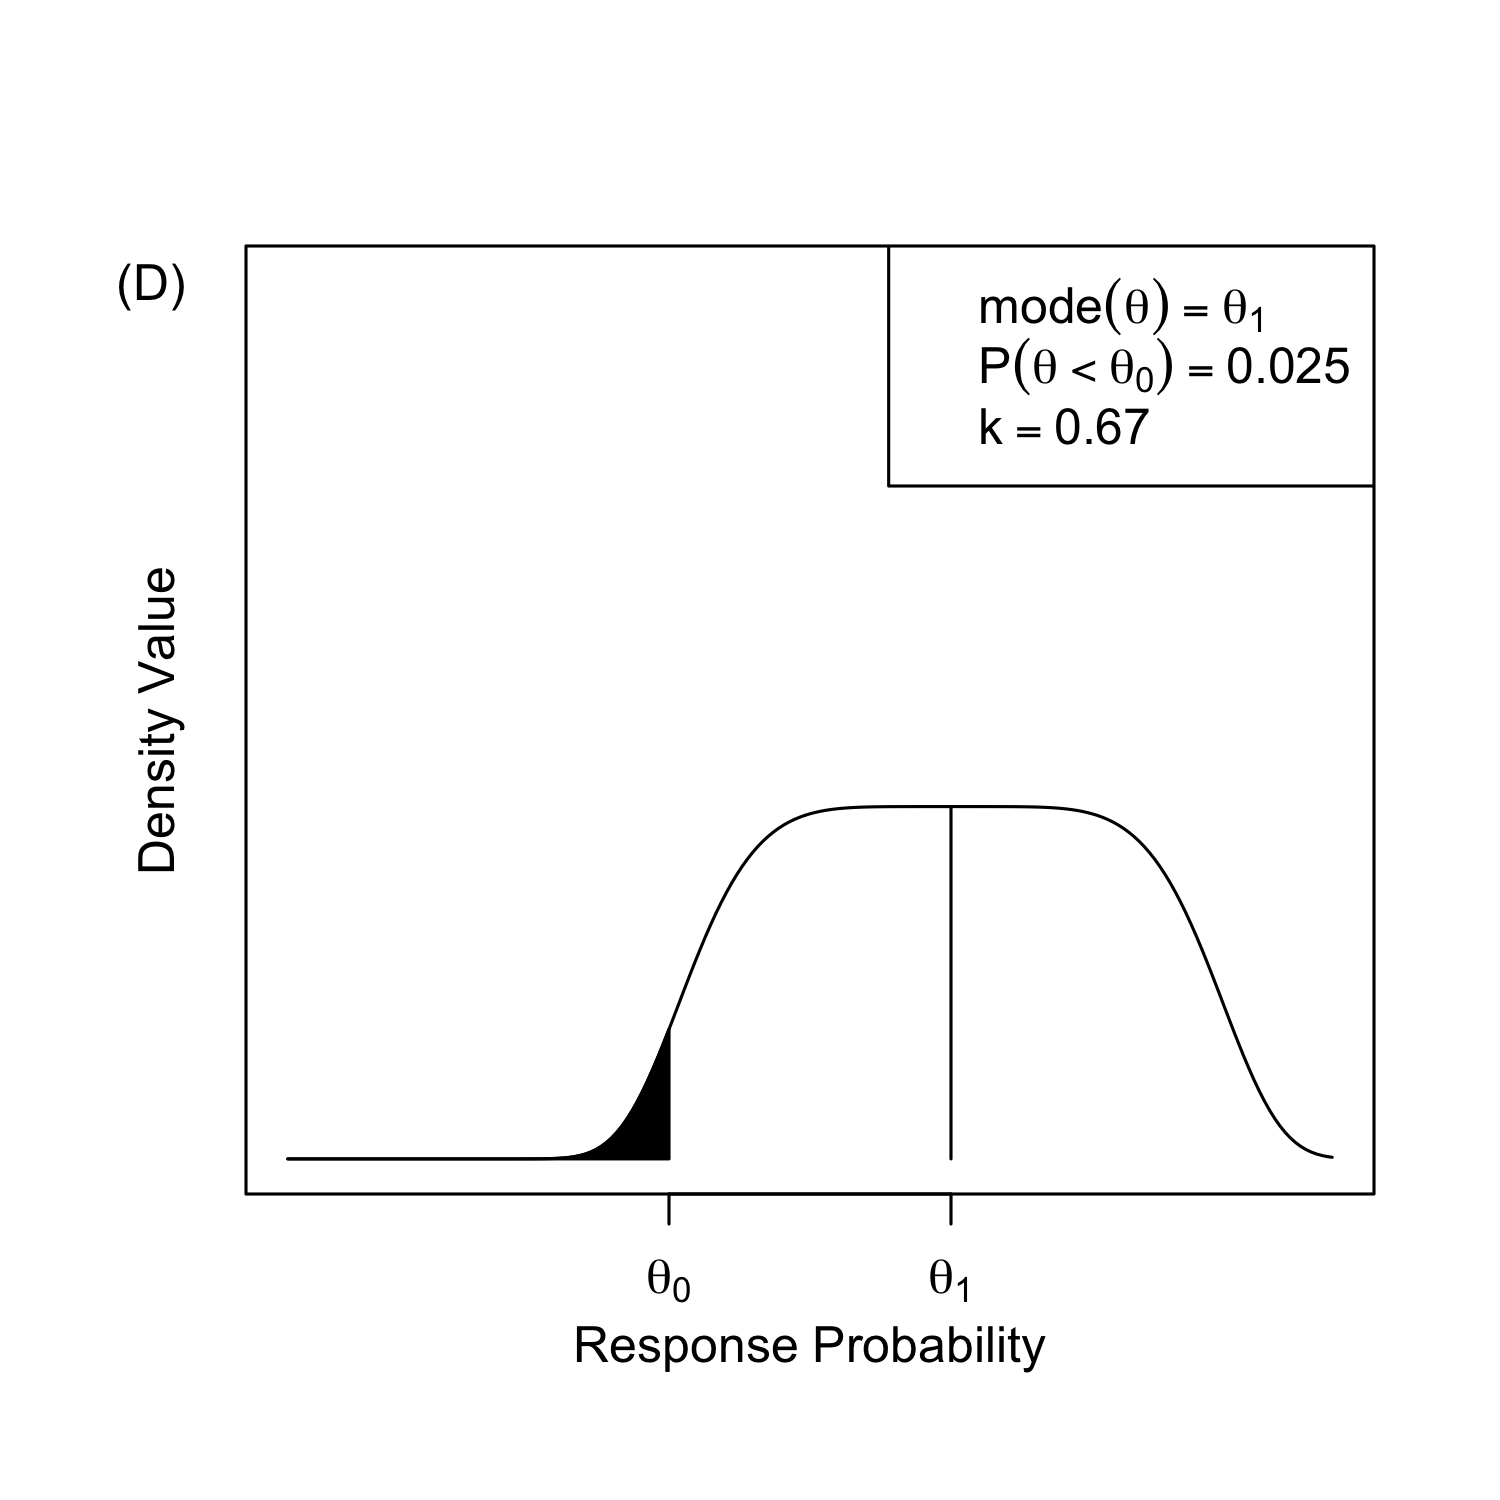
\includegraphics[width=0.5\textwidth]{./figures/figure1d.png}
\caption{C, Default enthusiastic prior. D, Flattened enthusiastic prior.}

\label{fig:figure1}
\end{center}
\end{figure}
\end{frame}

%\begin{frame}{Box's $p$-value}
%The prior-predictive distribution for data $\mathbf{D}$ (also called the marginal likelihood) reflects the probability of observing $\mathbf{D}$ given 
%the assumed prior distribution for $\theta$ and is defined formally as
%\begin{equation}\label{eq:pred_dist}
%p(\mathbf{D}) =\int p(\mathbf{D}|\theta)\pi(\theta)d\theta.
%\end{equation}
%	%
%Let $\mathbf{D}_{\text{obs}}$ be the observed data at some point in time in an ongoing trial. 
%	%
%\textit{Box's p-value} is defined as the following:
%%\begin{equation}
%%p=P(p(y)\leq p(y_{obs}))
%%\end{equation}
%\begin{equation}\label{eq:box_p}
%\psi({\mathbf{D}_{\text{obs}}})=\int {p(\mathbf{D})}  1[p(\mathbf{D})\leq p(\mathbf{D}_{\text{obs}})] d(\mathbf{D})
%%\sum_{\mathbf{D}}p^{(h)}(\mathbf{D})1[p^{(h)}(\mathbf{D})\leq p^{(h)}(\mathbf{D}_{\text{obs}})]
%\end{equation}
%%which in the case of discrete data is equal to $\psi({\mathbf{D}_{\text{obs}}})=\sum_{\mathbf{D}}p(\mathbf{D})1[p(\mathbf{D})\leq p(\mathbf{D}_{\text{obs}})]$.
%%
%where $1[A]$ is an indicator that the event $A$ is true.
%\end{frame}

\begin{frame}{Adaptive Monitoring Prior}
\begin{itemize}
\item Let $\mathbf{D}_{\text{obs}}$ be the observed data at some point in time in an ongoing trial, and let $p(\mathbf{D}) =\int p(\mathbf{D}|\theta)\pi(\theta)d\theta$ be the prior-predictive distribution for the data.

	%
\item \textit{Box's p-value} is defined as the following:

\begin{equation}\label{eq:box_p}
\psi({\mathbf{D}_{\text{obs}}})=\int {p(\mathbf{D})}  1[p(\mathbf{D})\leq p(\mathbf{D}_{\text{obs}})] d(\mathbf{D})
%\sum_{\mathbf{D}}p^{(h)}(\mathbf{D})1[p^{(h)}(\mathbf{D})\leq p^{(h)}(\mathbf{D}_{\text{obs}})]
\end{equation}

\item 
We define the \textit{adaptive monitoring prior} \textcolor{black}{for efficacy evaluations} as the mixture distribution	
\begin{equation}\label{eq:inference_prior}
	\pi_{AE}\left(\theta\right)=\omega\cdot\pi_E(\theta)+(1 - \omega)\cdot \pi_S(\theta)
\end{equation}
\item
Define the mixing weight $\omega$ given to the \textit{enthusiastic} prior as
\begin{align}\label{eq:omega}
\omega= \psi^{(E)}(\mathbf{D}_{\text{obs}})
\end{align}
%\item This mixture weight achieves the goal of favoring the enthusiastic component if the trial data are compatible with that prior, and otherwise assigning a higher weight to the skeptical component. 
%\item The minimum possible mixing weight $\delta$ assigned to the \textit{skeptical} prior is achieved when $\psi^{(E)}(\mathbf{D}_{\text{obs}})=1$ and is equal to $\delta$. 
%\item Choices of $\delta$ in $\{0, 0.05, 0.10, 0.15, 0.20, 0.25\}$ are explored.
\end{itemize}
\end{frame}



\begin{frame}{PLUTO Trial}
\begin{itemize}
\item
We consider the trial ``The Pediatric Lupus Trial of Belimumab Plus Background Standard Therapy (PLUTO)" (NCT01649765) which was conducted between September 2012 and January 2018 \citep{Brunner2020}.
\item
The primary endpoint was a dichotomous variable reflecting a 4-point or greater reduction in SELENA SLEDAI score from baseline to week 52. 
\item External data is used to identify $\eta_0=0.39$, $\theta_1=0.12$, using $\theta_0=0$ as the null value.
\item A frequentist two-sided hypothesis test with confidence level $95\%$ and $80\%$ power would require 266 patients per group.
\end{itemize}
\end{frame}


%\begin{frame}{Simulation Plan}
%\begin{itemize}
%\item A maximum sample size of $n_{\text{max}}=100$ was chosen based on the original trial protocol.
%\item 
%A minimum sample size of $n_{min}=50$ was chosen to provide an adequate number of placebo controls to be enrolled given the initial 5:1 allocation to the treatment group.
%\item 
%An interim analysis is completed after every two patients have outcomes beginning at $n_{min}$.
%\item Placebo response rate generated at $39\%$
%\end{itemize}
%\end{frame}



%\begin{frame}
%\begin{figure}[htbp]
%\begin{center}
%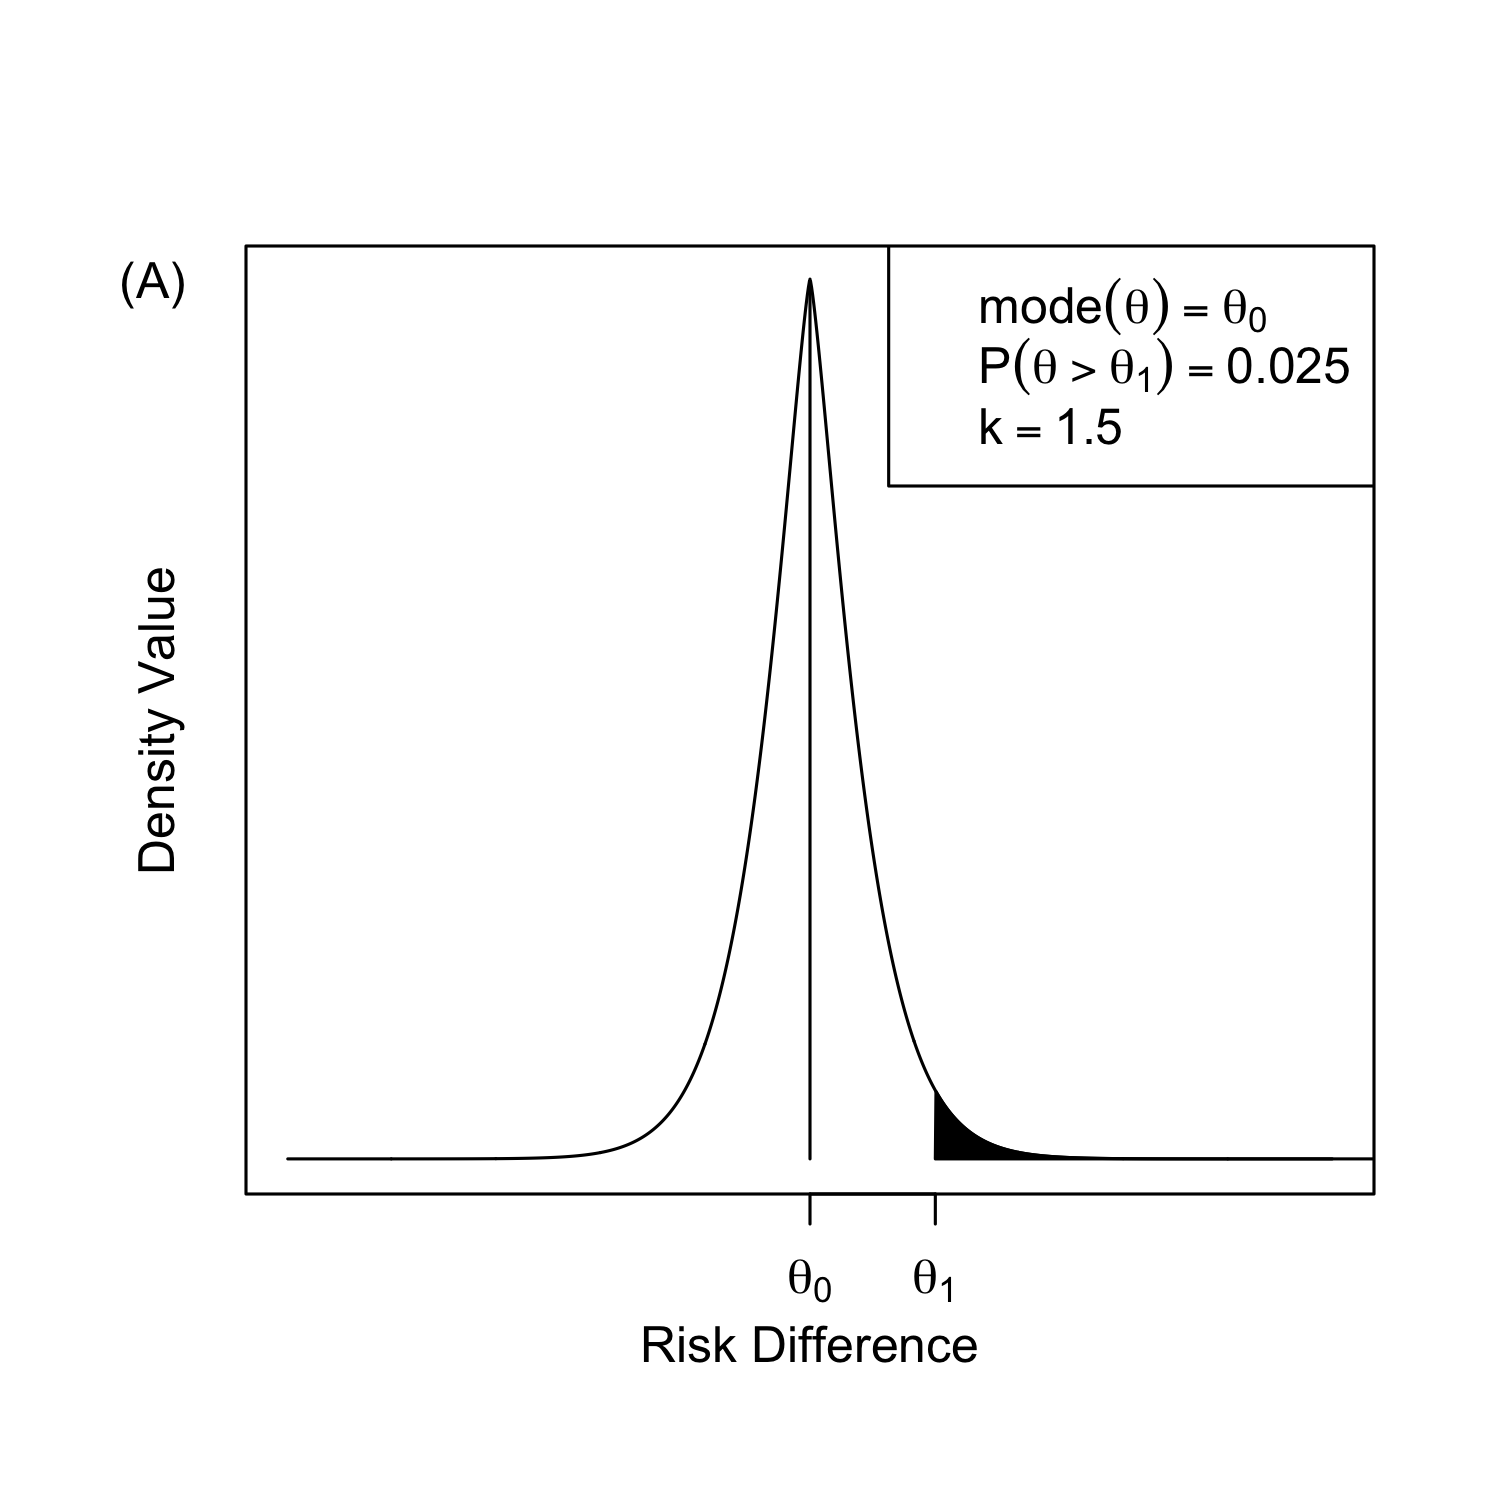
\includegraphics[width=0.5\textwidth]{./figures/figure5a_NEW.png}%
%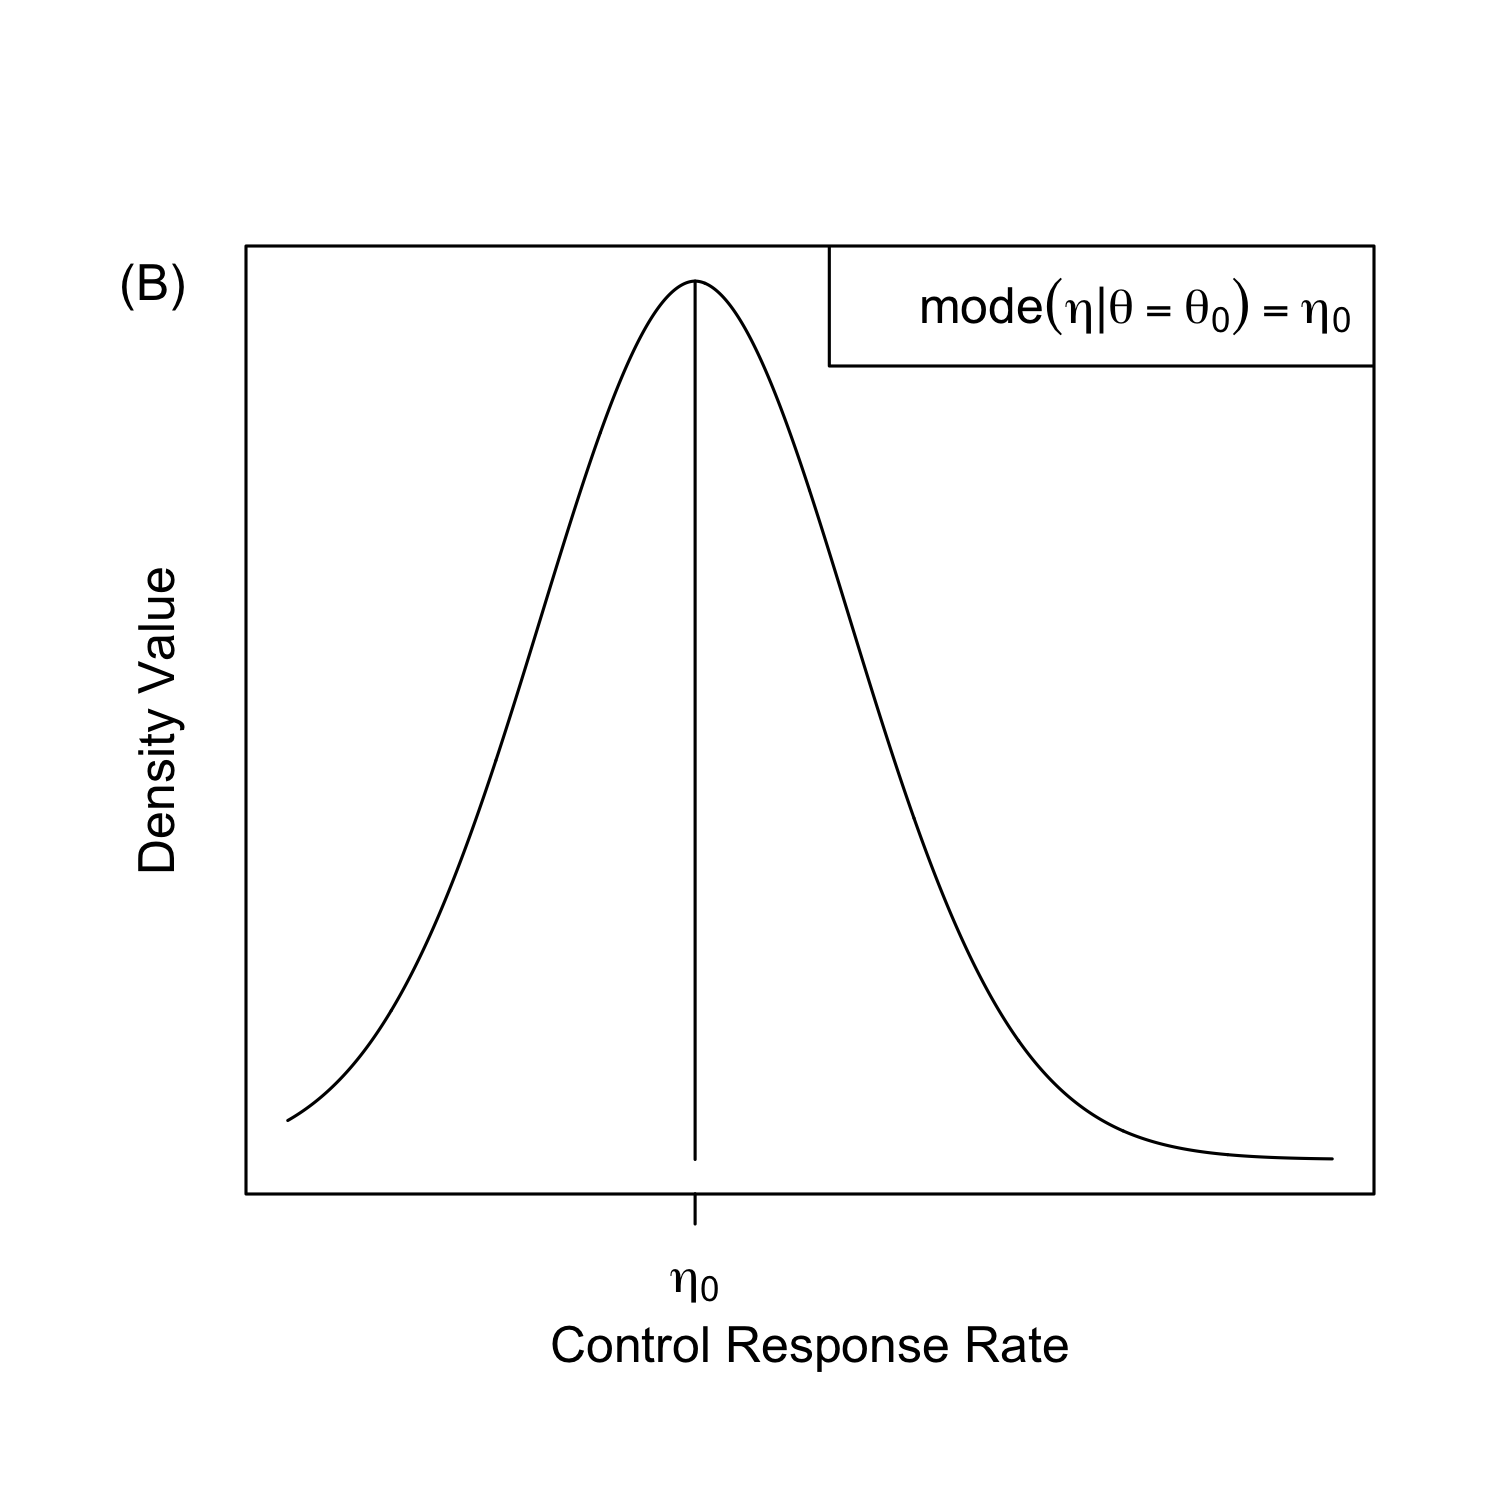
\includegraphics[width=0.5\textwidth]{./figures/figure5b_NEW.png}
%\caption{A, Concentrated skeptical prior $\pi_S(\theta)$ truncated to $[-1,1]$. B, Conditional prior $\pi(\eta|\theta=\theta_0)$.}
%\label{fig:figure5}
% \end{center}
%\end{figure}
%\end{frame}
%
%\begin{frame}{Joint Enthusiastic Monitoring Prior}
%\begin{figure}[htbp]
%\begin{center}
%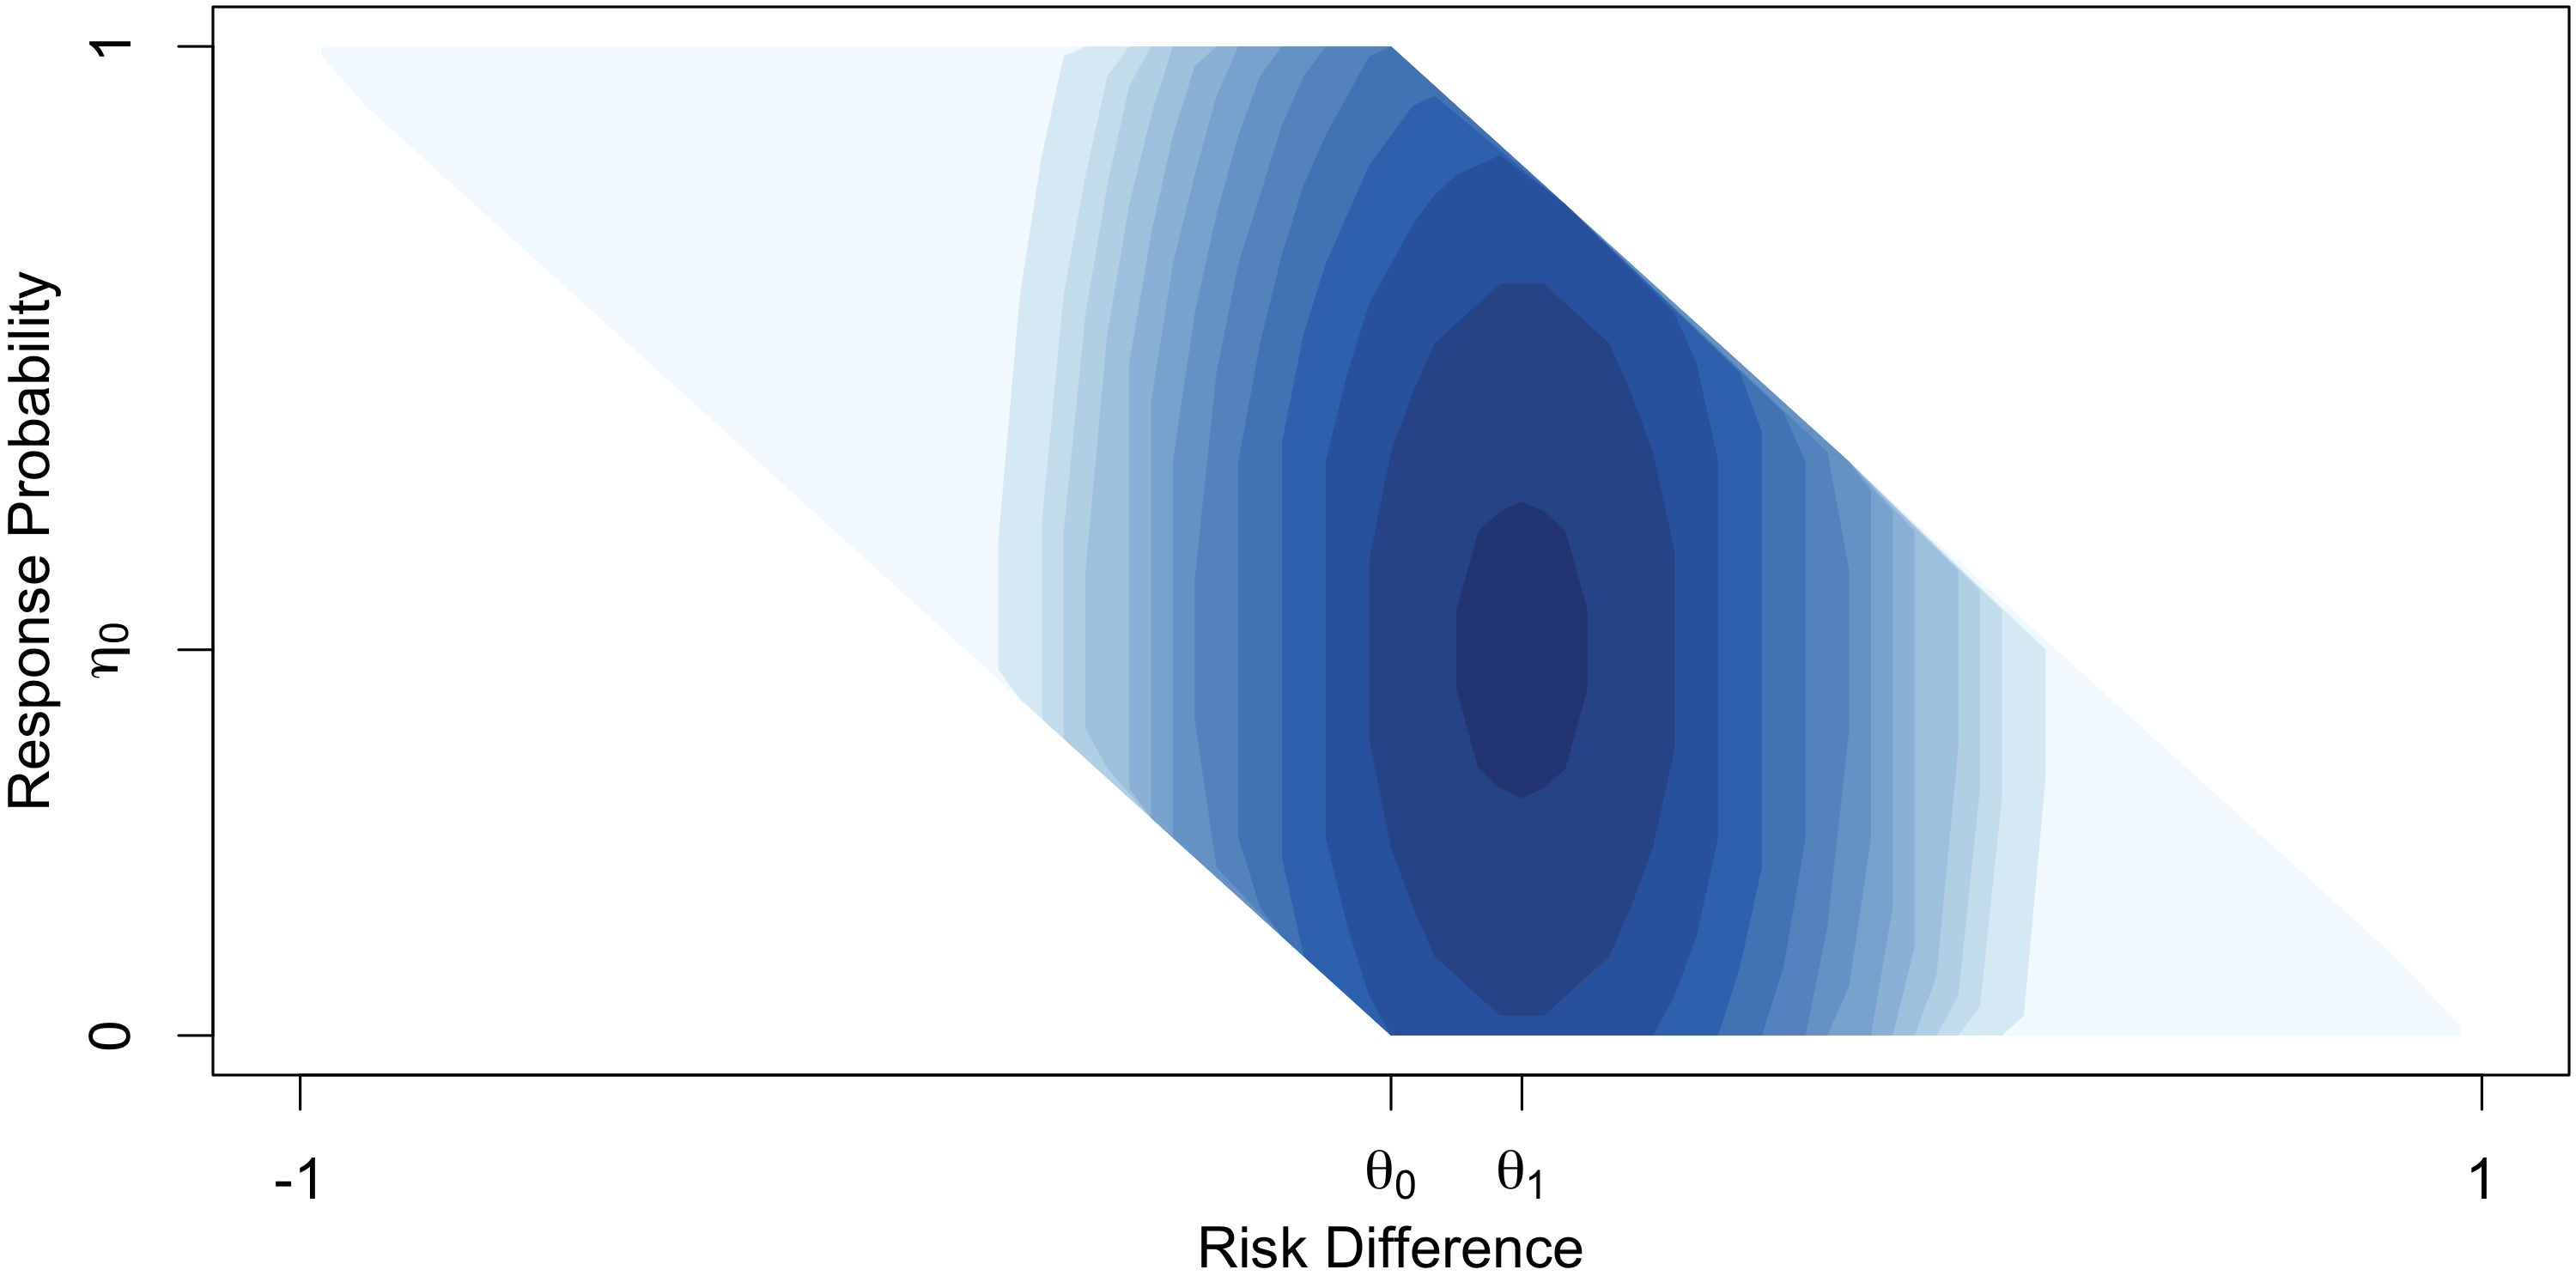
\includegraphics[width=1\textwidth]{./figures/enth_aug12.png}
%\caption{Joint prior $\pi(\theta,\eta)=\pi(\theta)\times\pi(\eta|\theta)$ truncated based on the conditions $-1<\theta<1$ and $0<\theta+\eta<1$.}
%\label{fig:figure5}
% \end{center}
%\end{figure}
%\end{frame}



%\begin{frame}
%\begin{figure}[htbp]
%\begin{center}
%    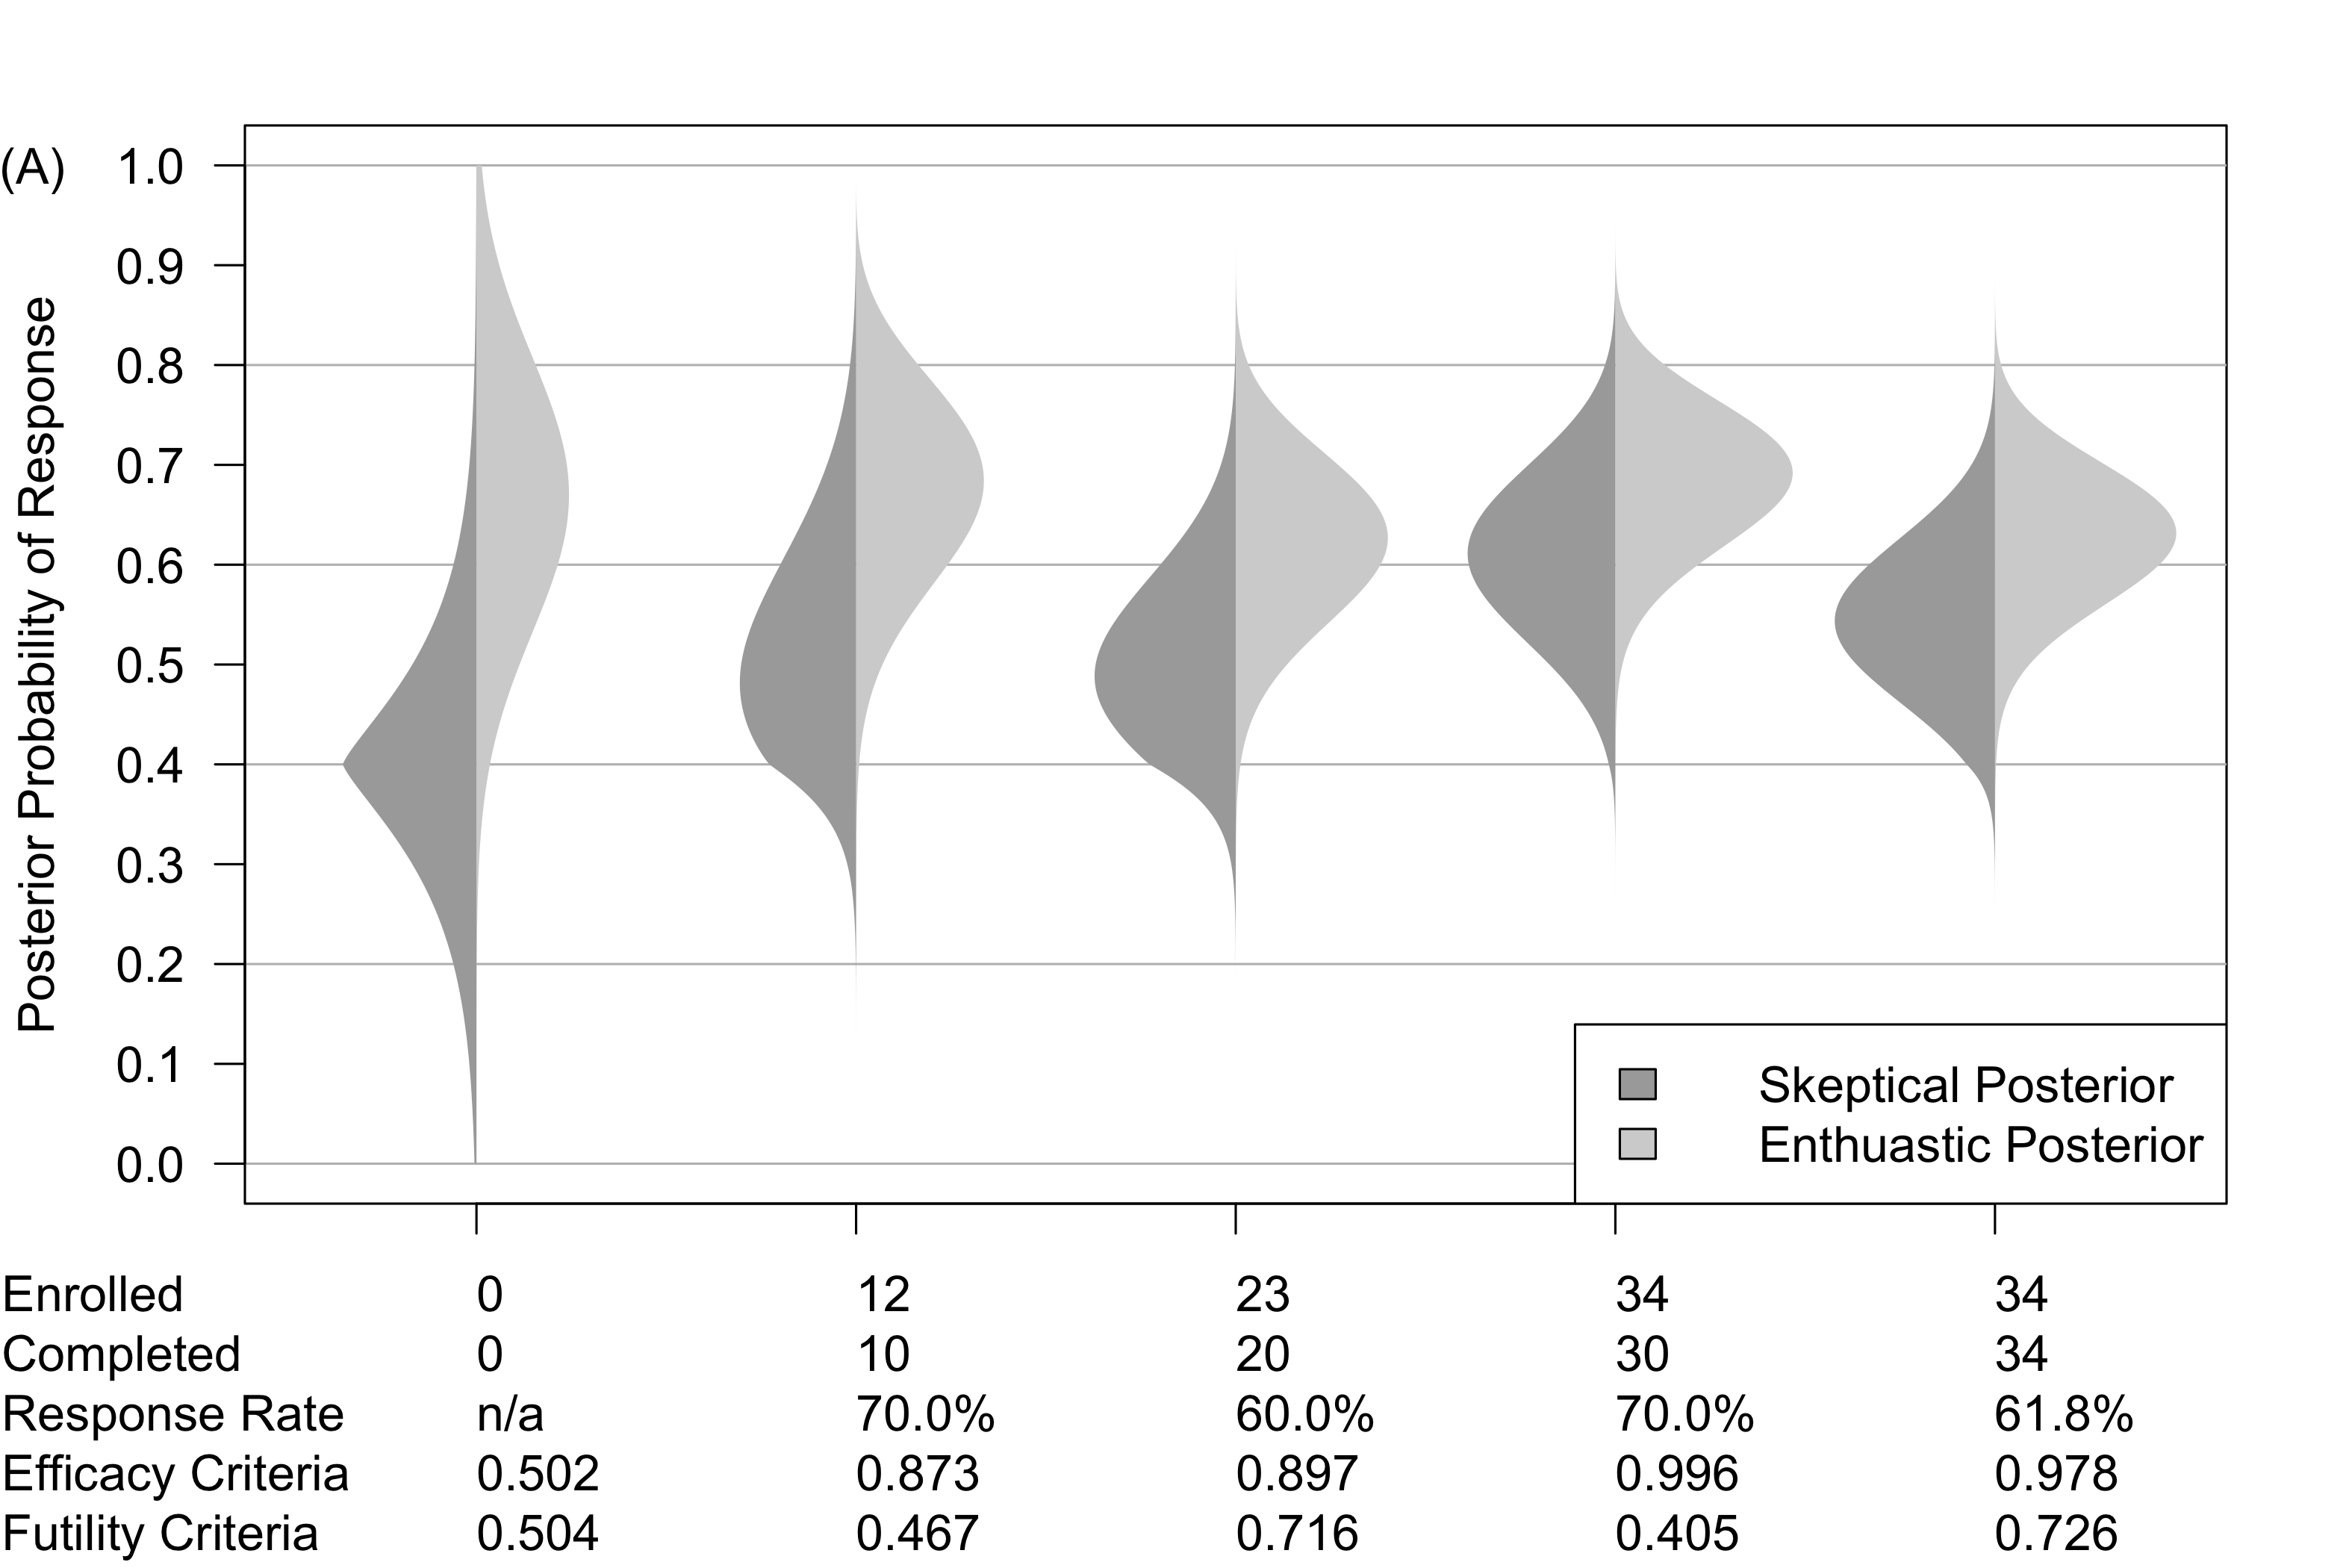
\includegraphics[width=1in]{./figures/figure2a.png}
%    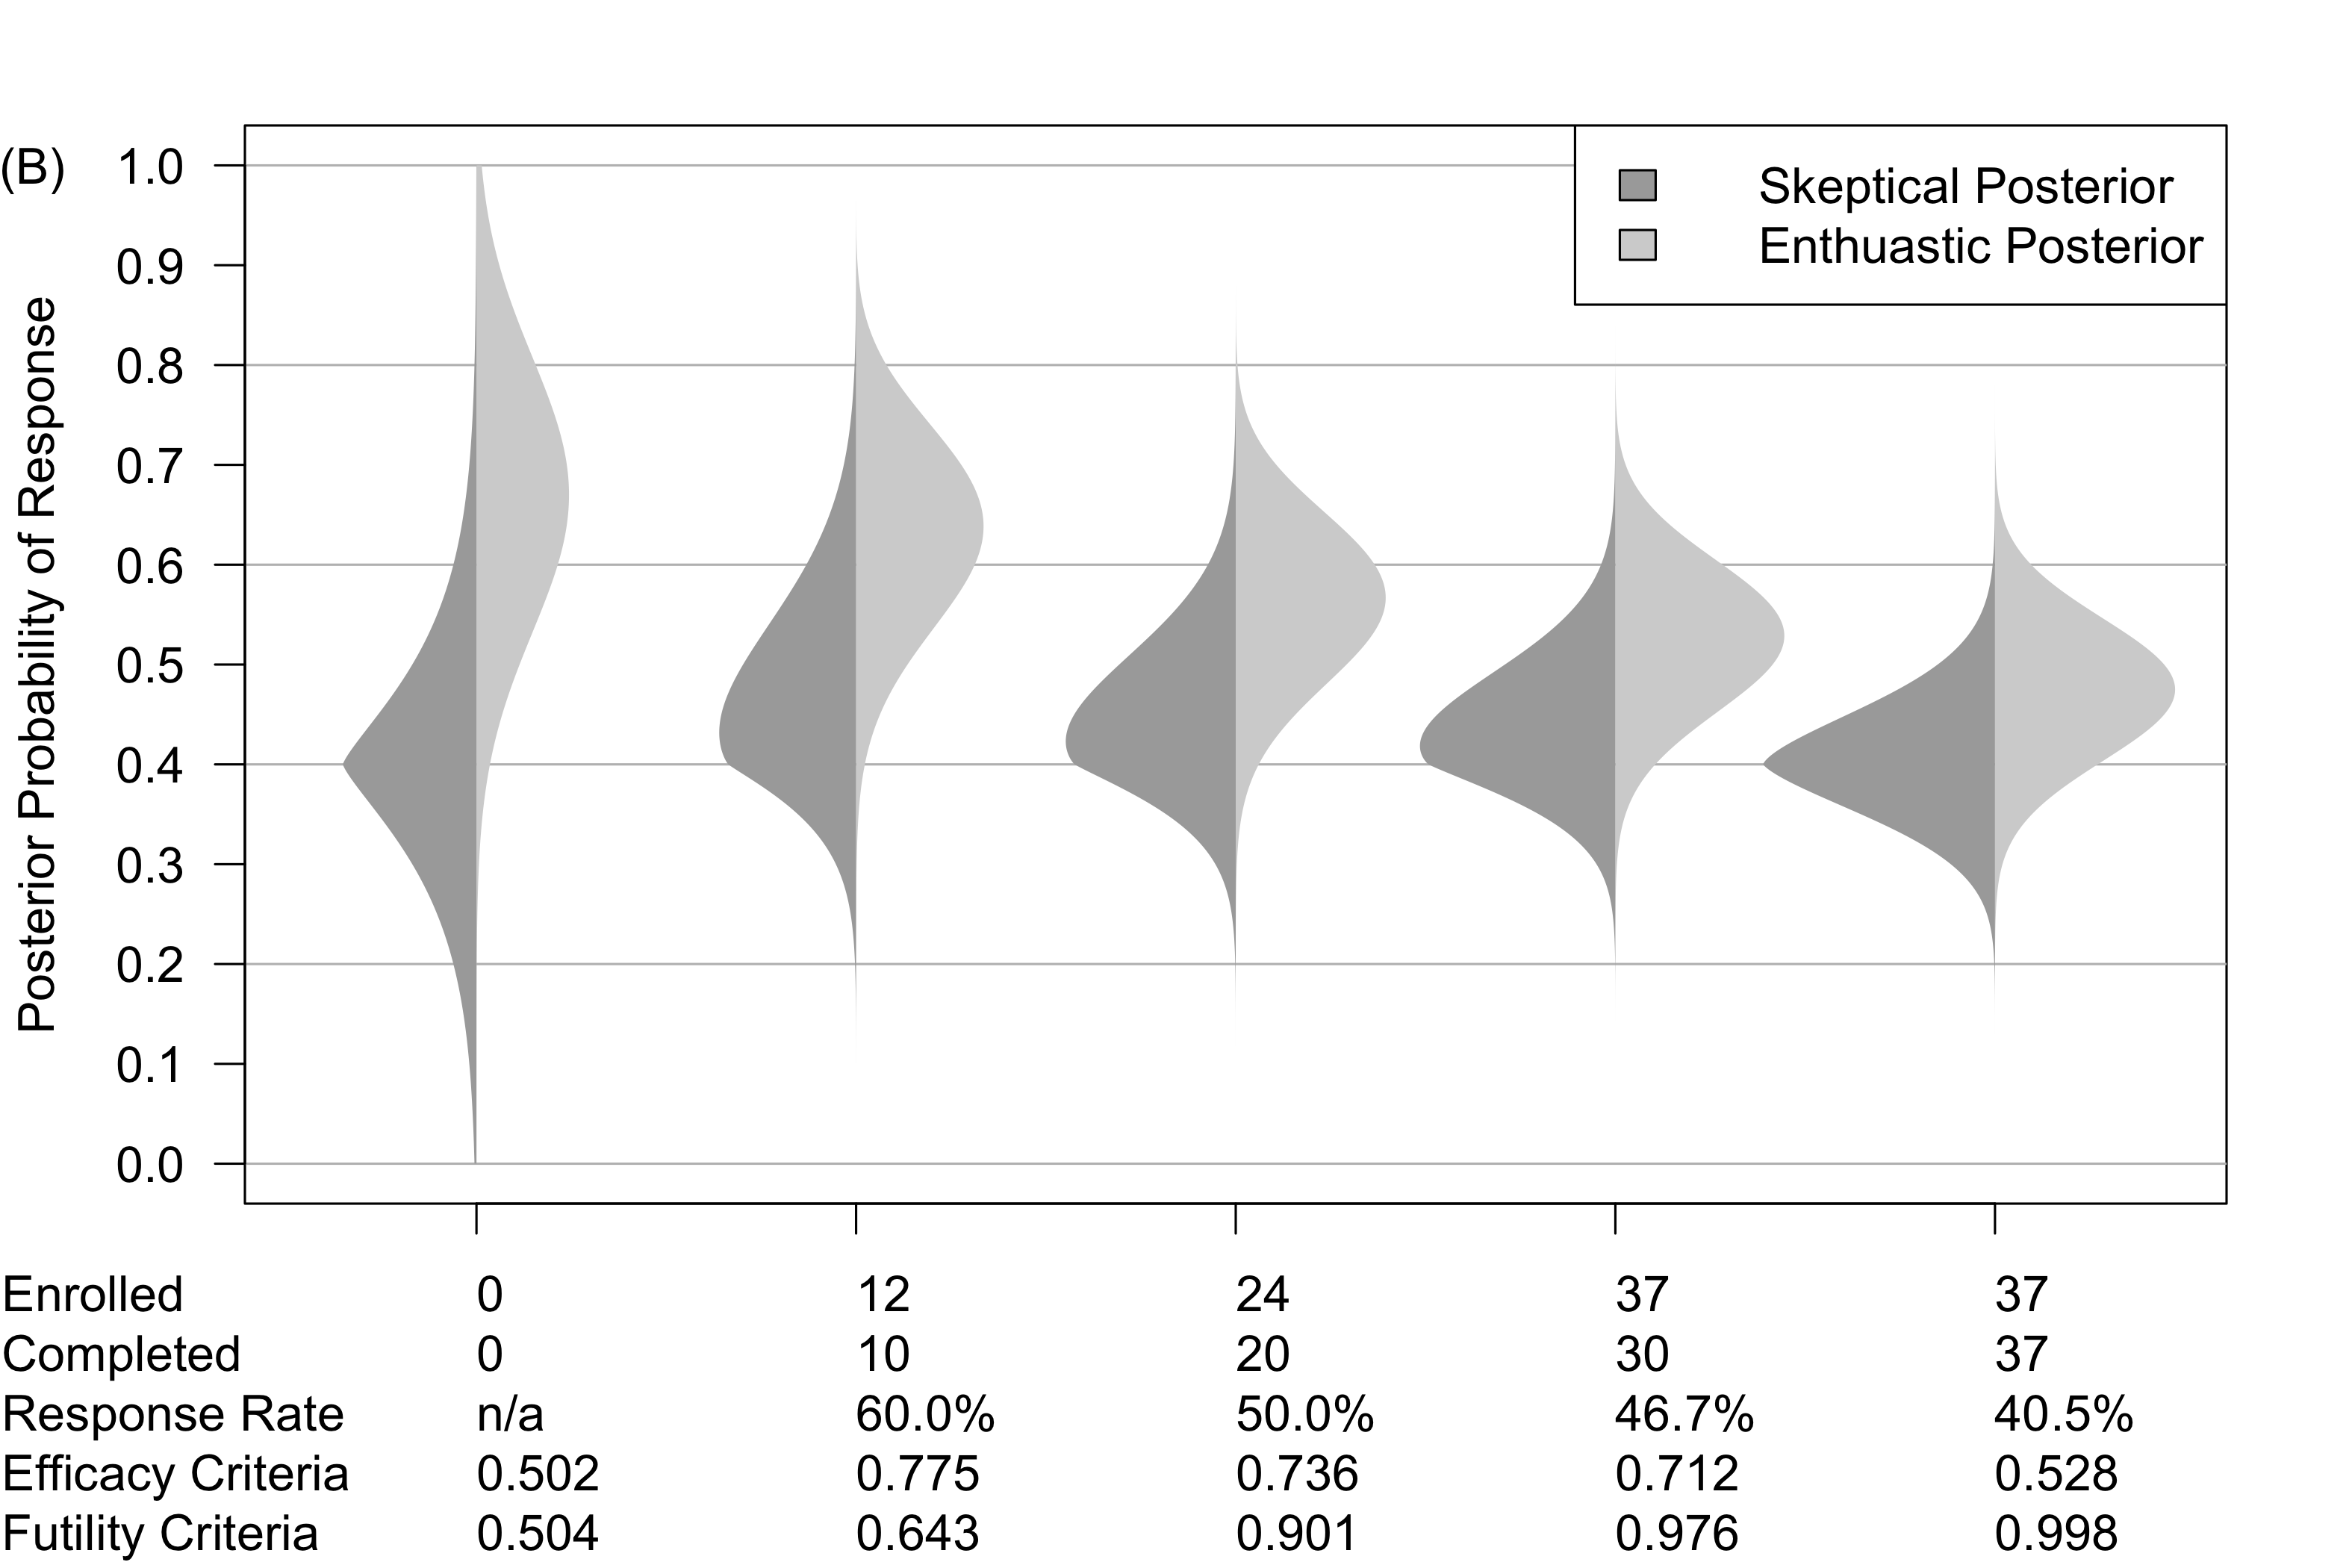
\includegraphics[width=1in]{./figures/figure2b.png}
%    \caption{Example paths for the trial described in Section \ref{sec:example1model}. A, Early stoppage for efficacy. B, Early stoppage for futility.}
%	\label{fig:figure2}
%\end{center}
%\end{figure}
%\end{frame}

%\begin{frame}
%\begin{figure}[htbp]
%\begin{center}
%
%    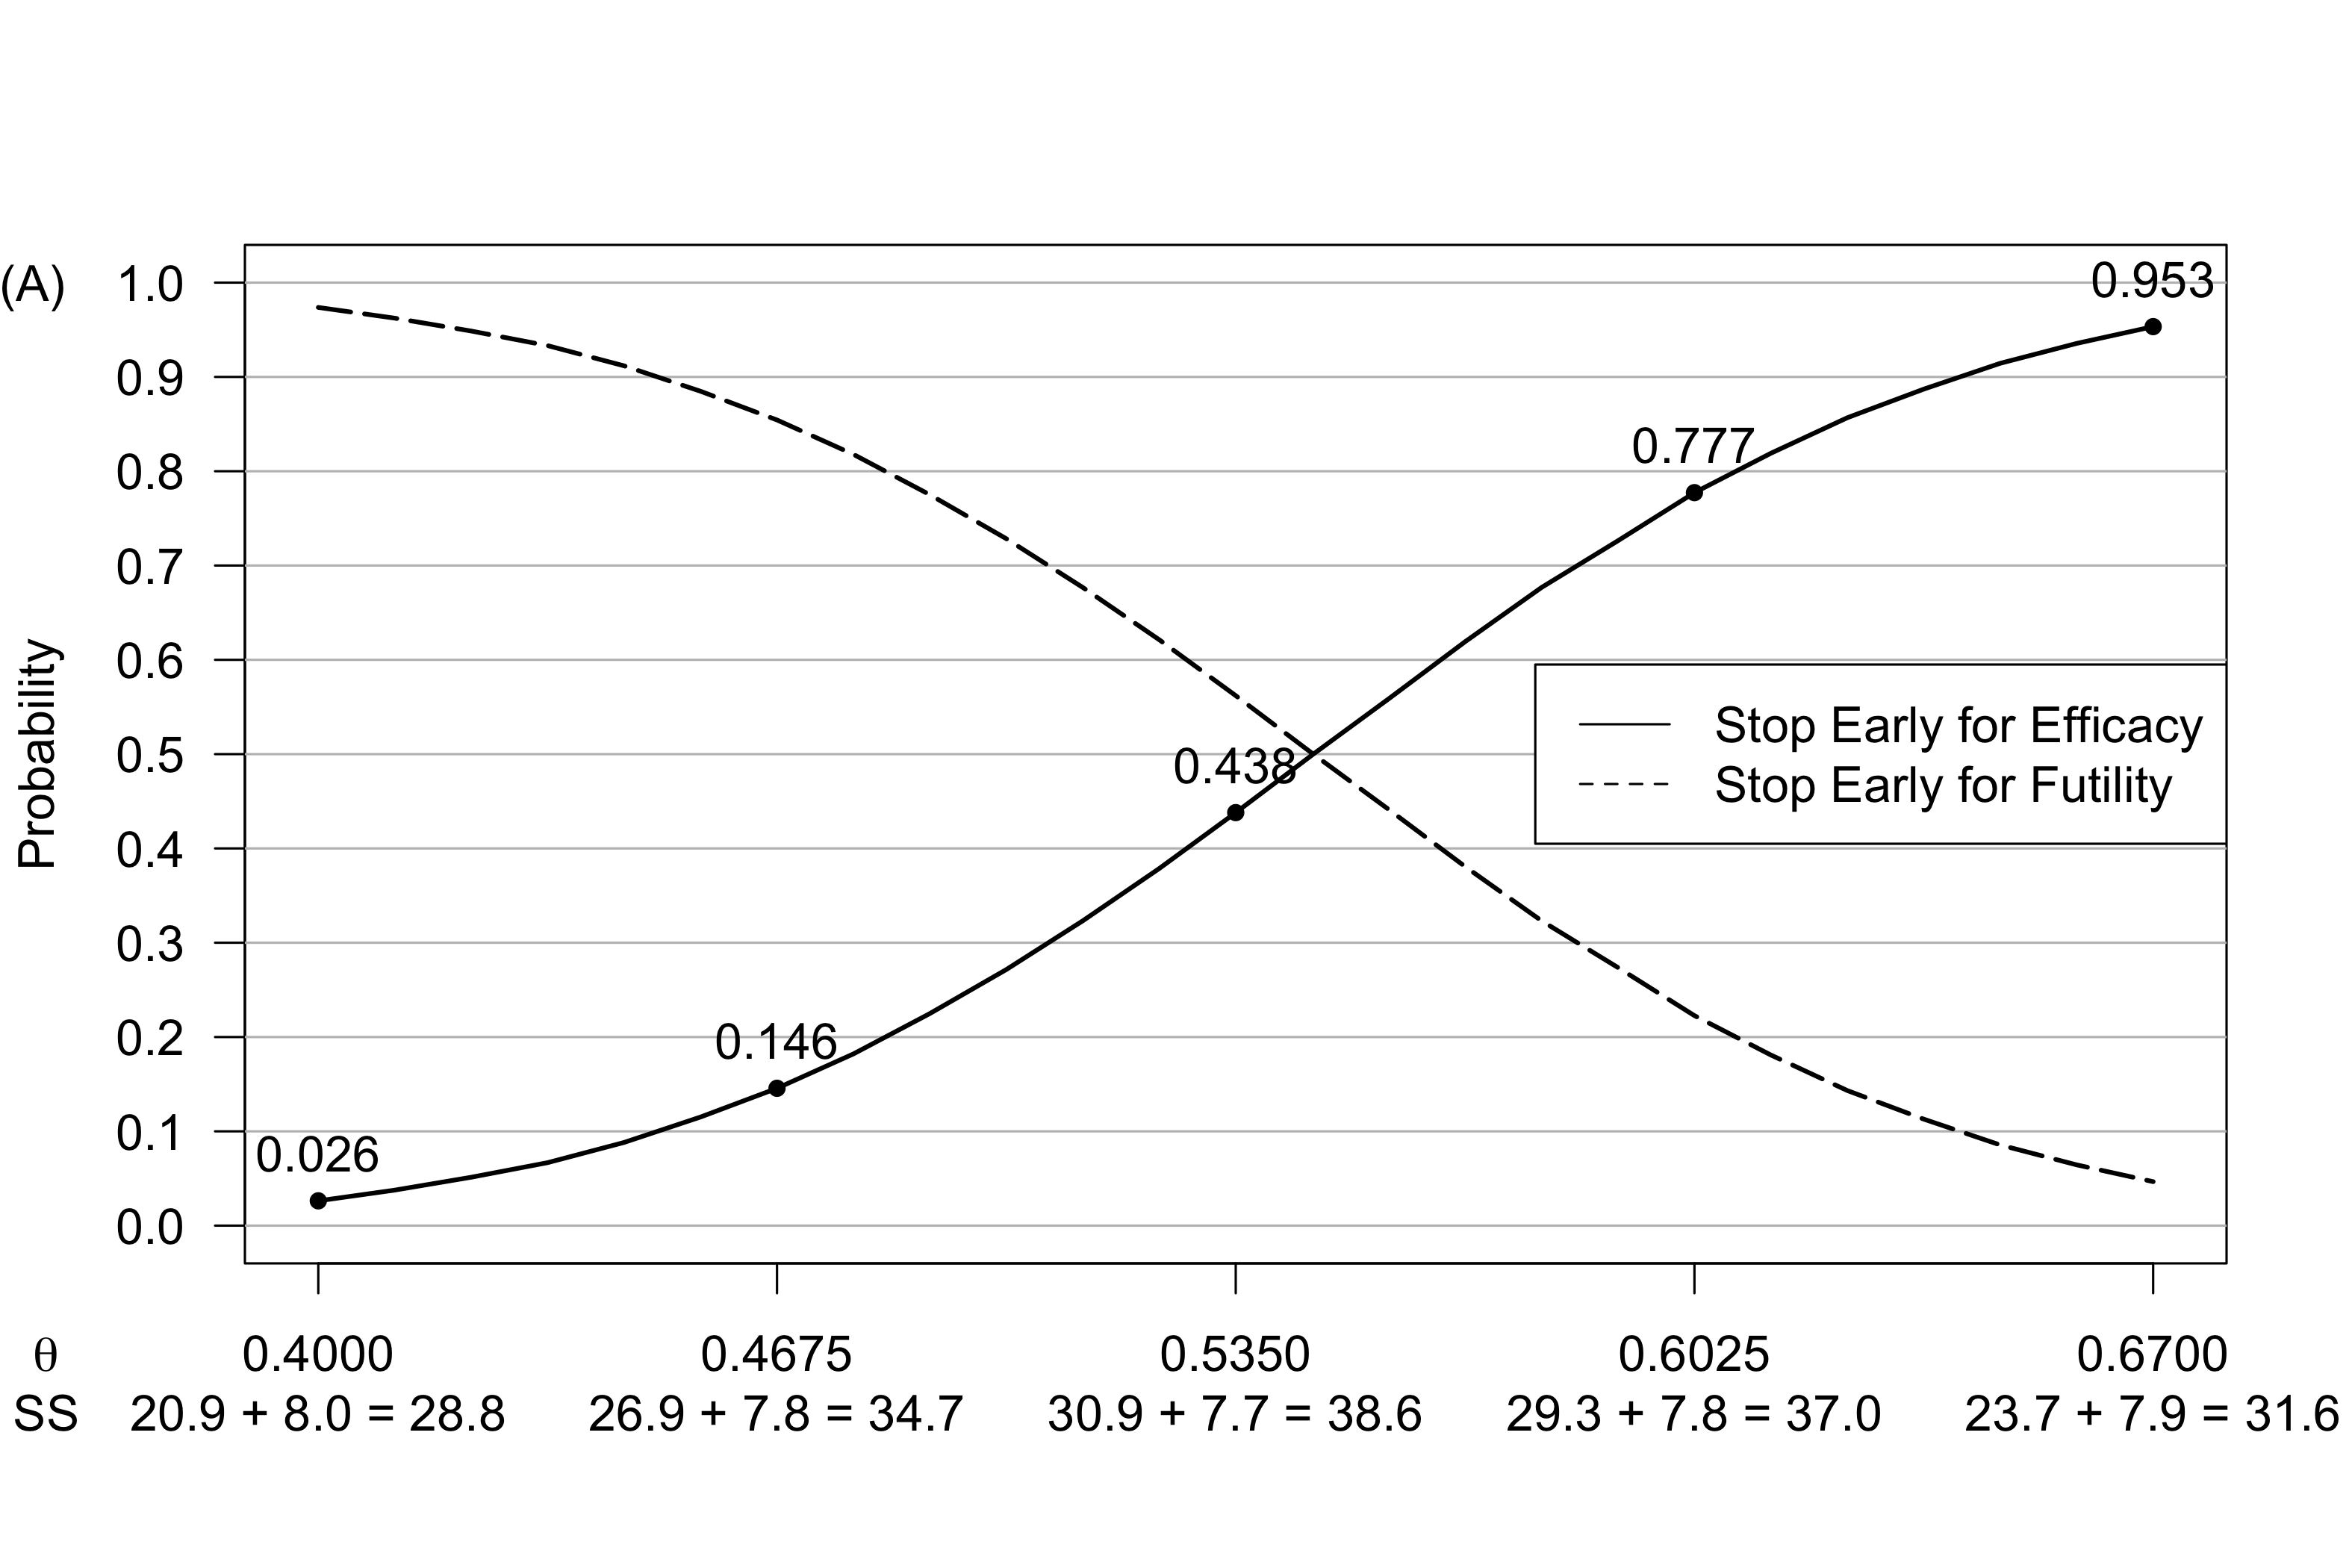
\includegraphics[width=1in]{./figures/figure3a.png}
%    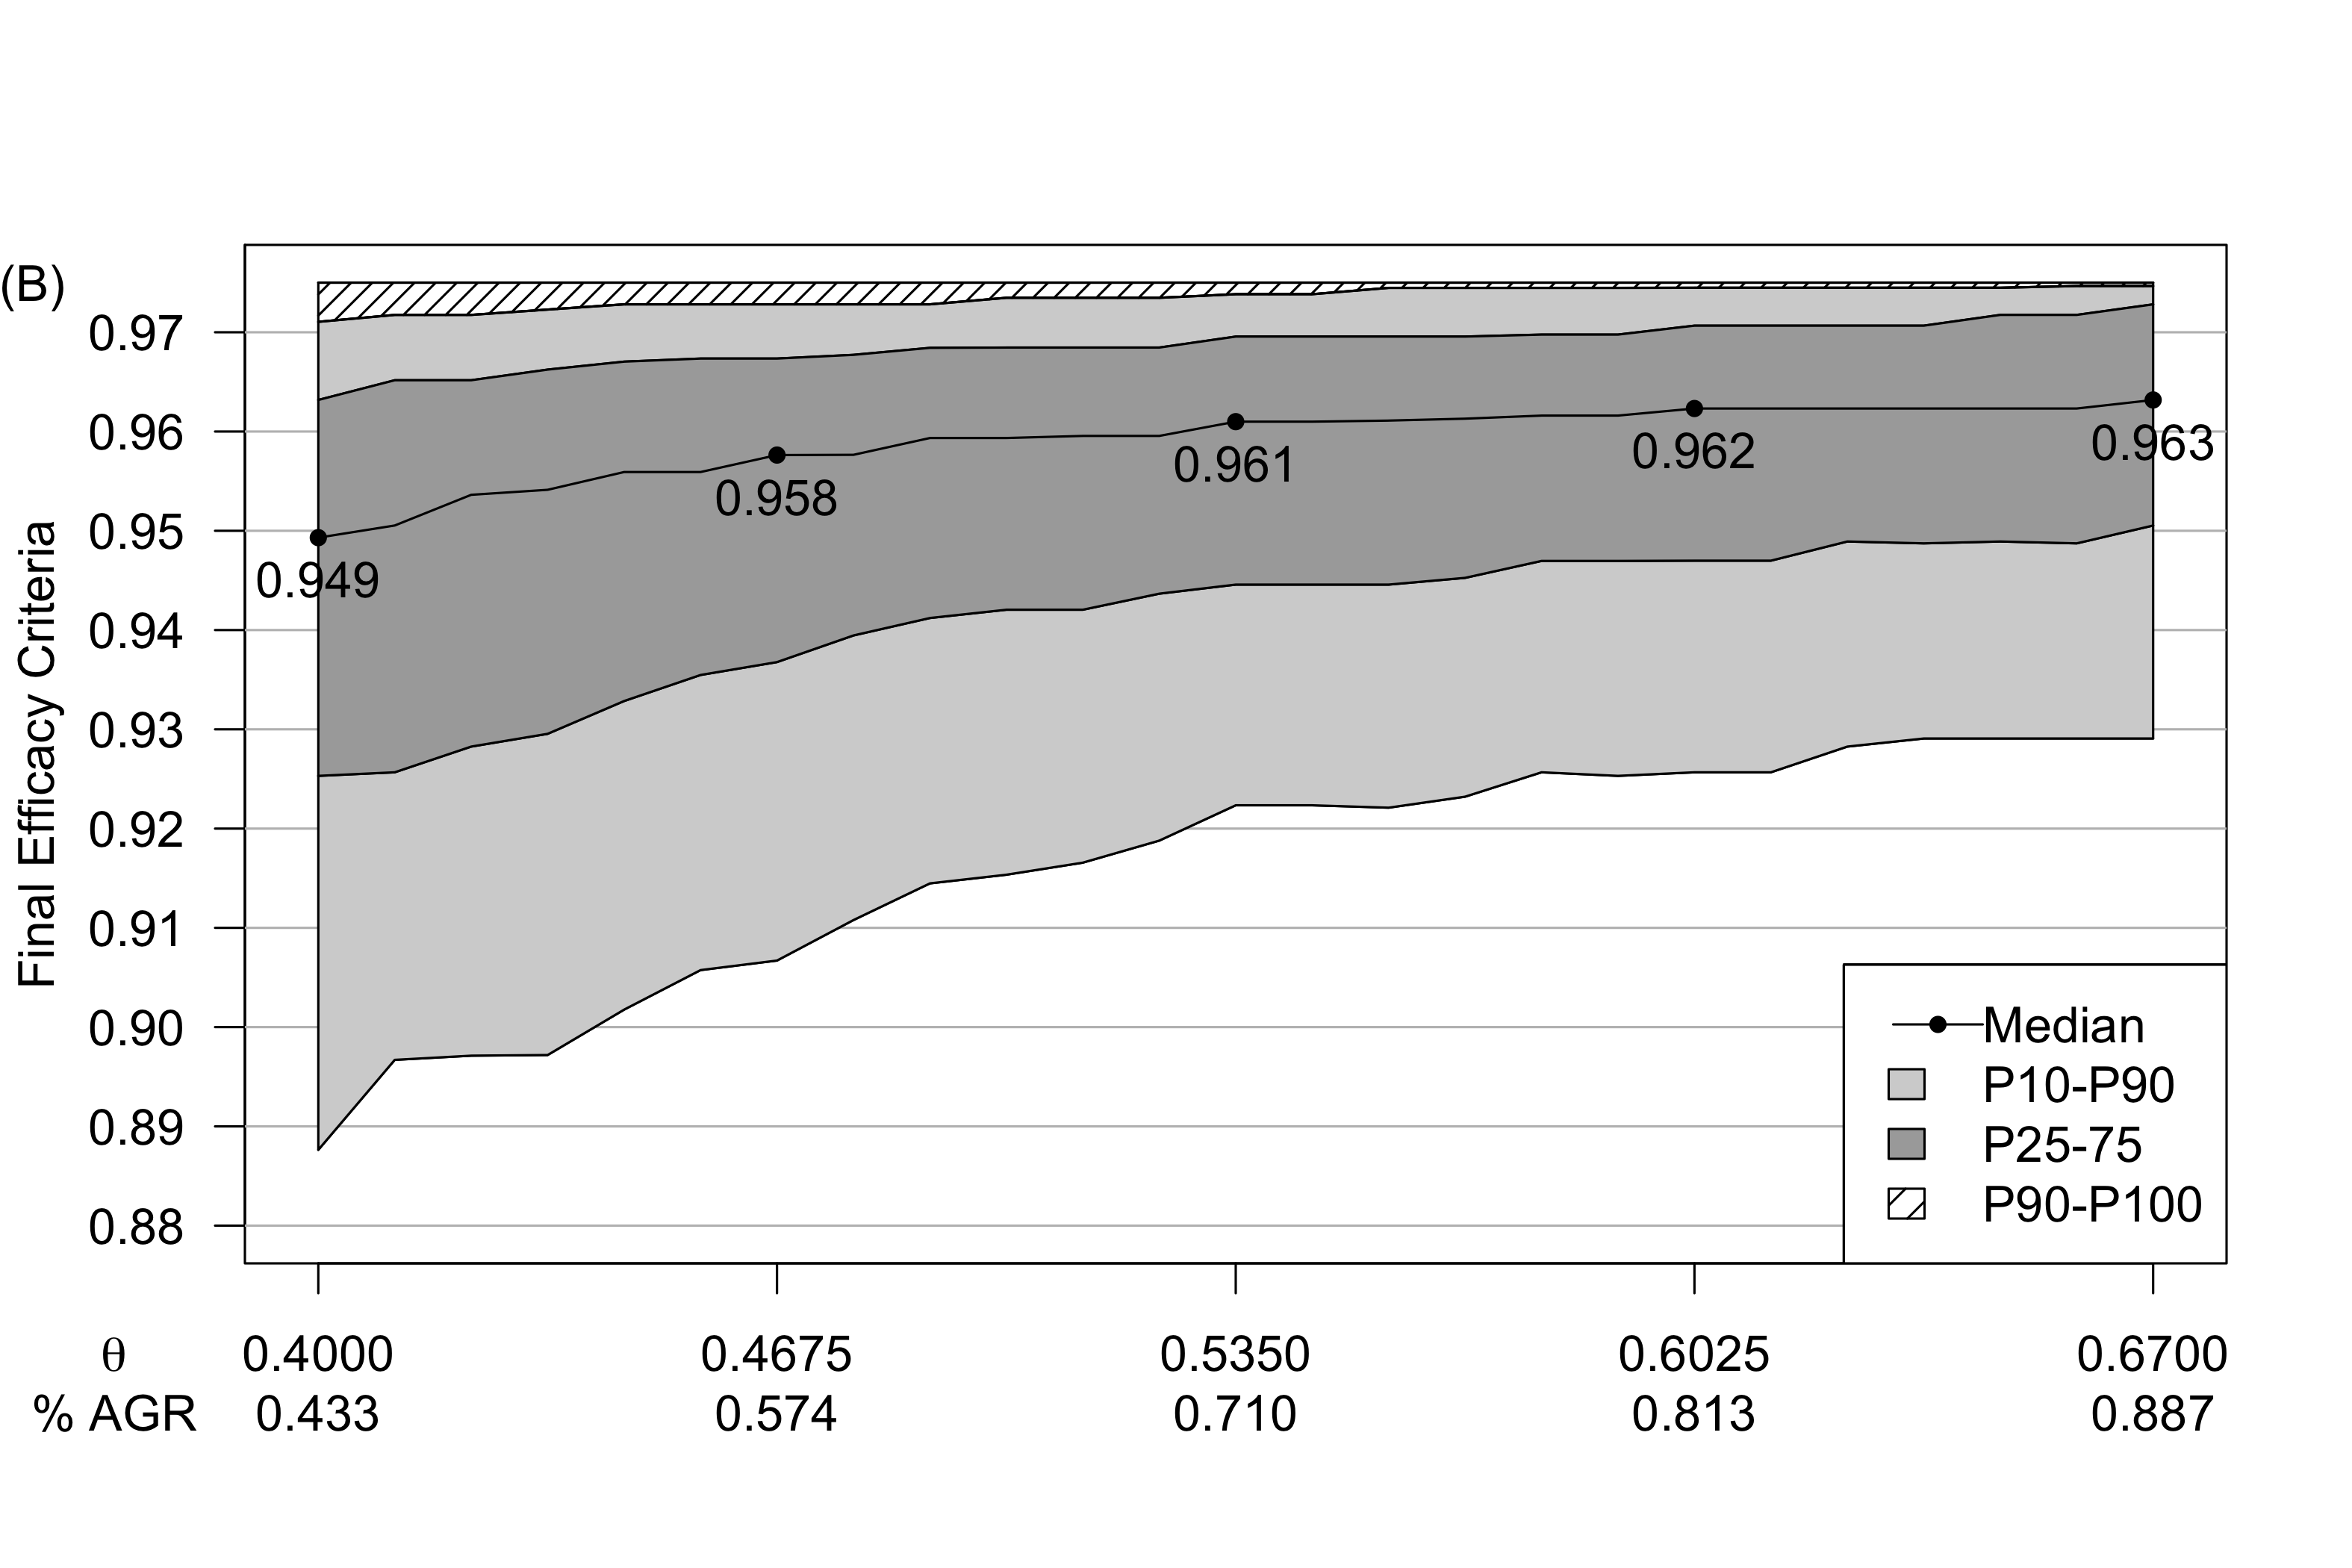
\includegraphics[width=1in]{./figures/figure3b.png}
%    \caption{A, Sequential design properties. (SS; mean sample size, (I); interim analysis, (F); final analysis). B, Distribution of final posterior probability given interim stoppage and evidence decrease ($\%$ AGR; percent of agreement between final and interim posterior probabilities relative to $1-\epsilon$ threshold).}
%	\label{fig:ex1.1}
%
%\end{center}
%\end{figure}
%\end{frame}

%\begin{frame}{Enthusiastic Prior Mixing Weight $\omega$}
%\begin{figure}[htbp]
%\begin{center}
%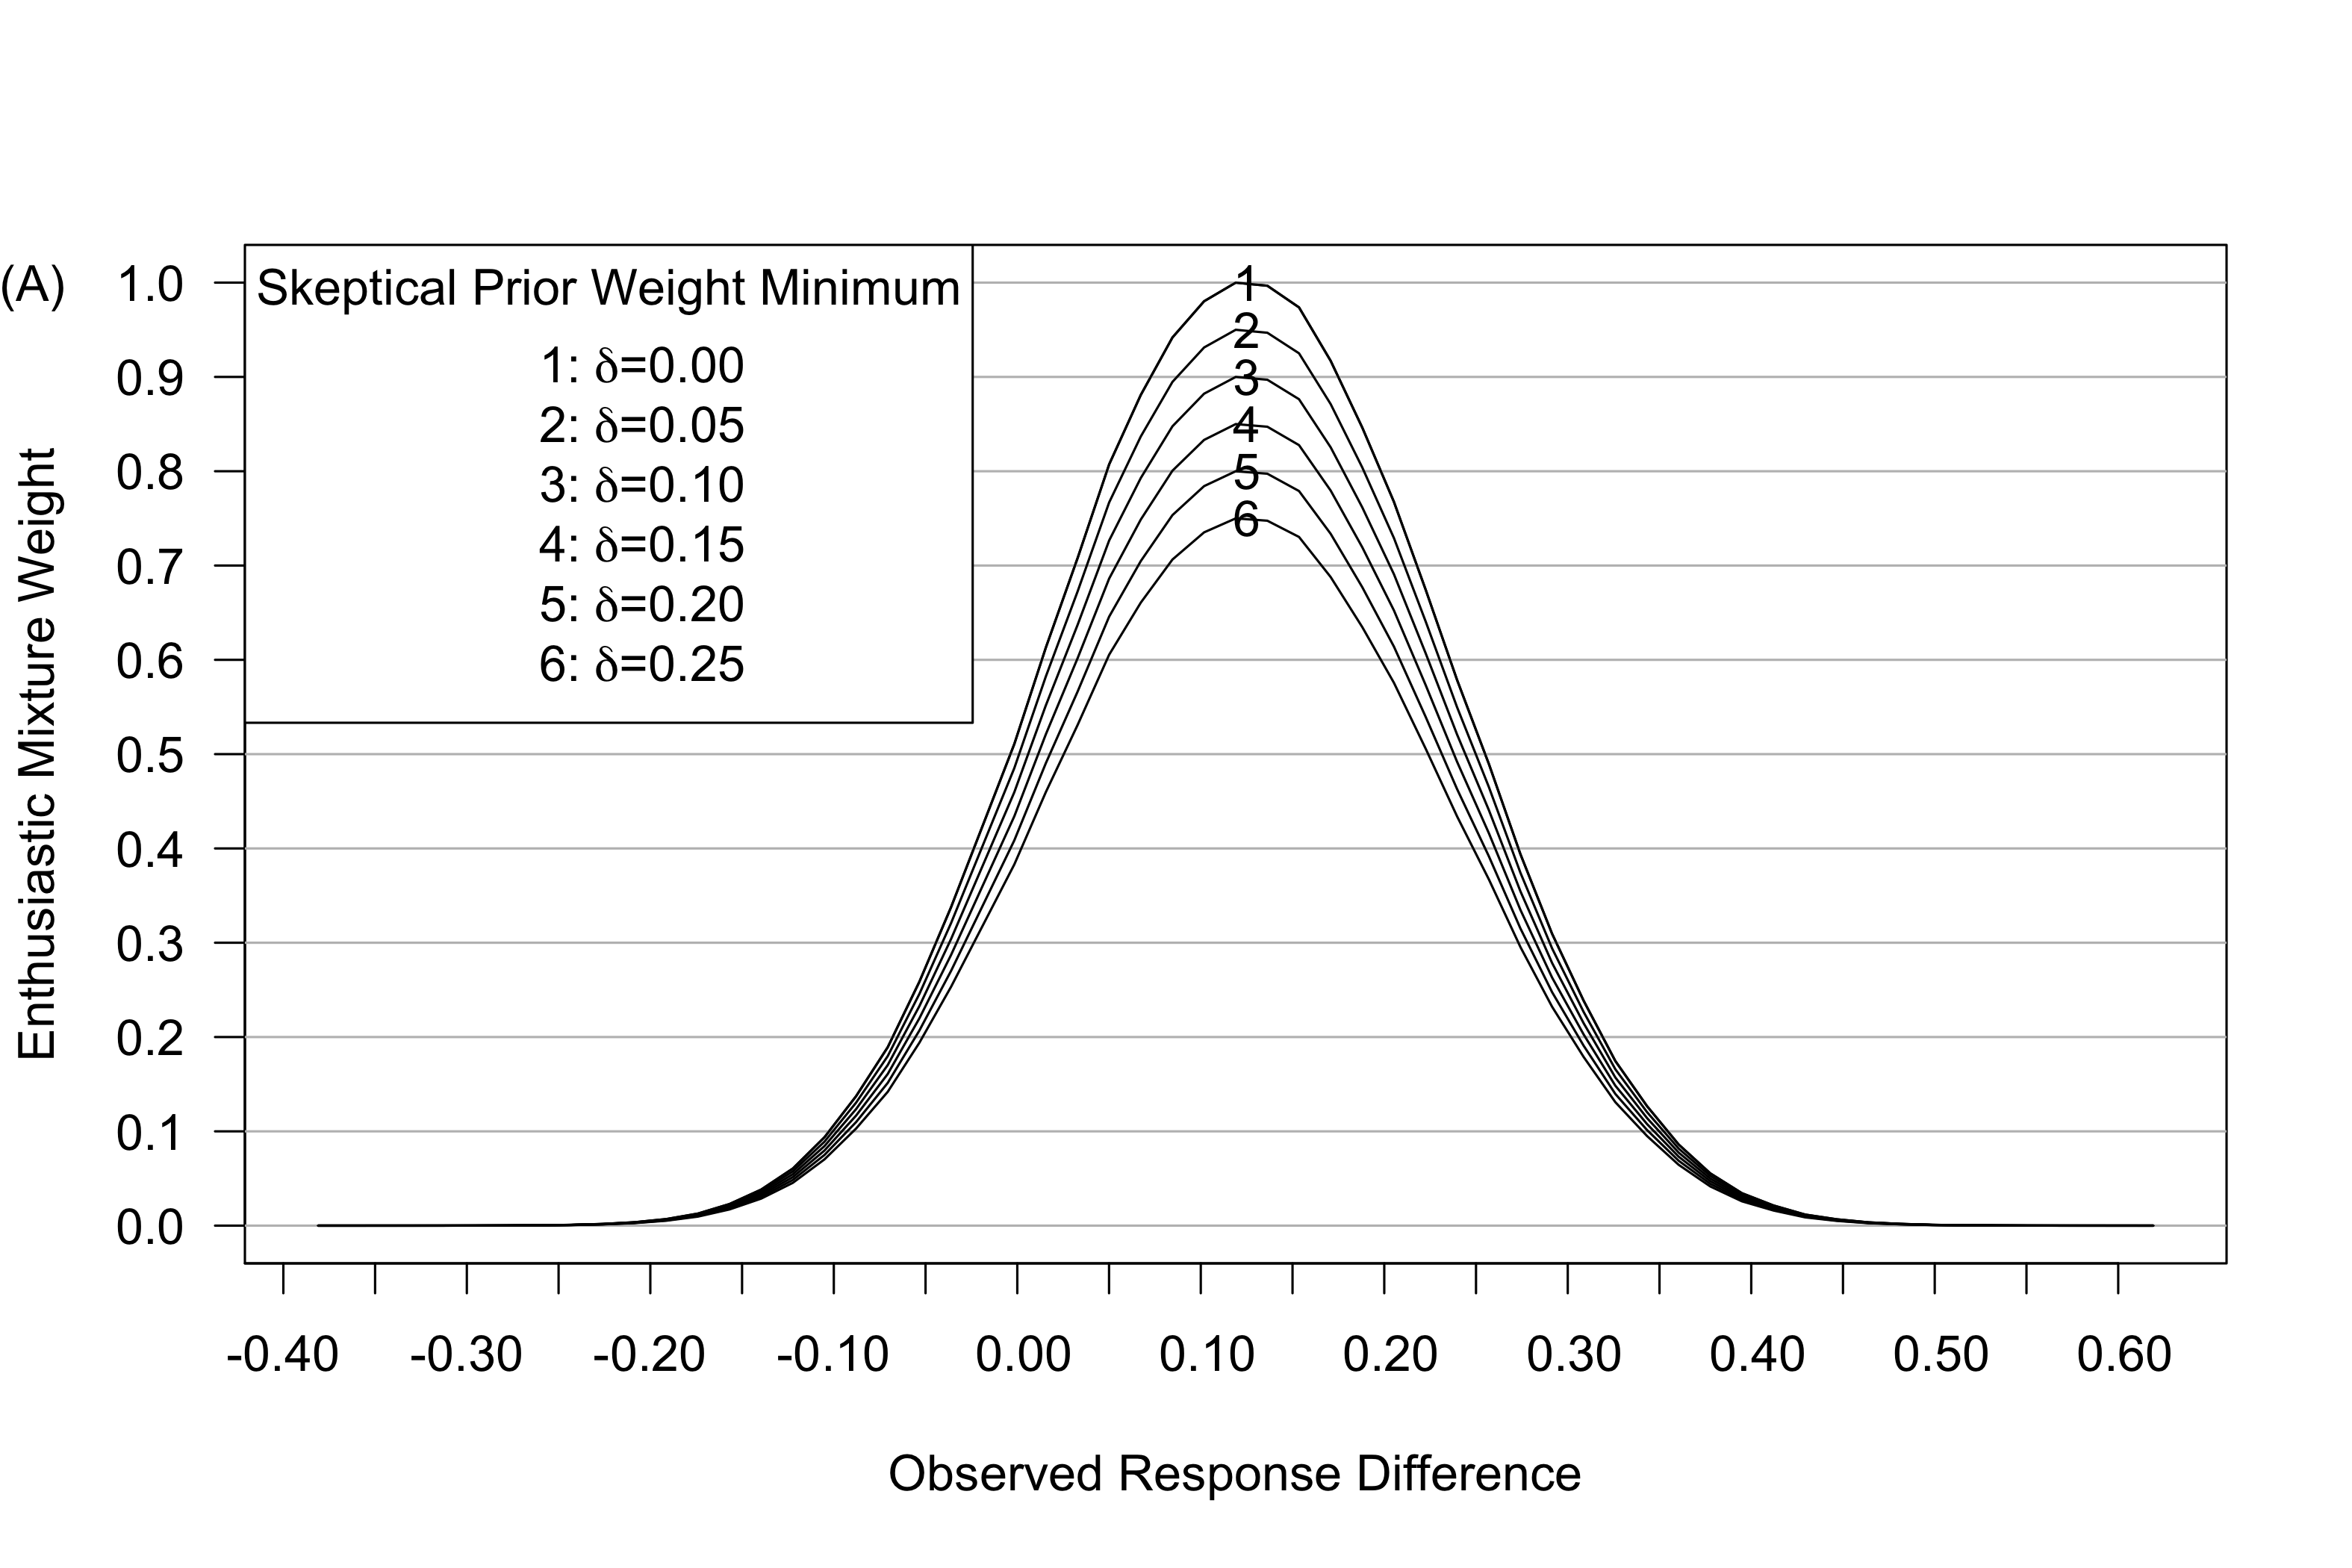
\includegraphics[width=0.8\textwidth]{./figures/3-part-compatibility-2.png}
%%    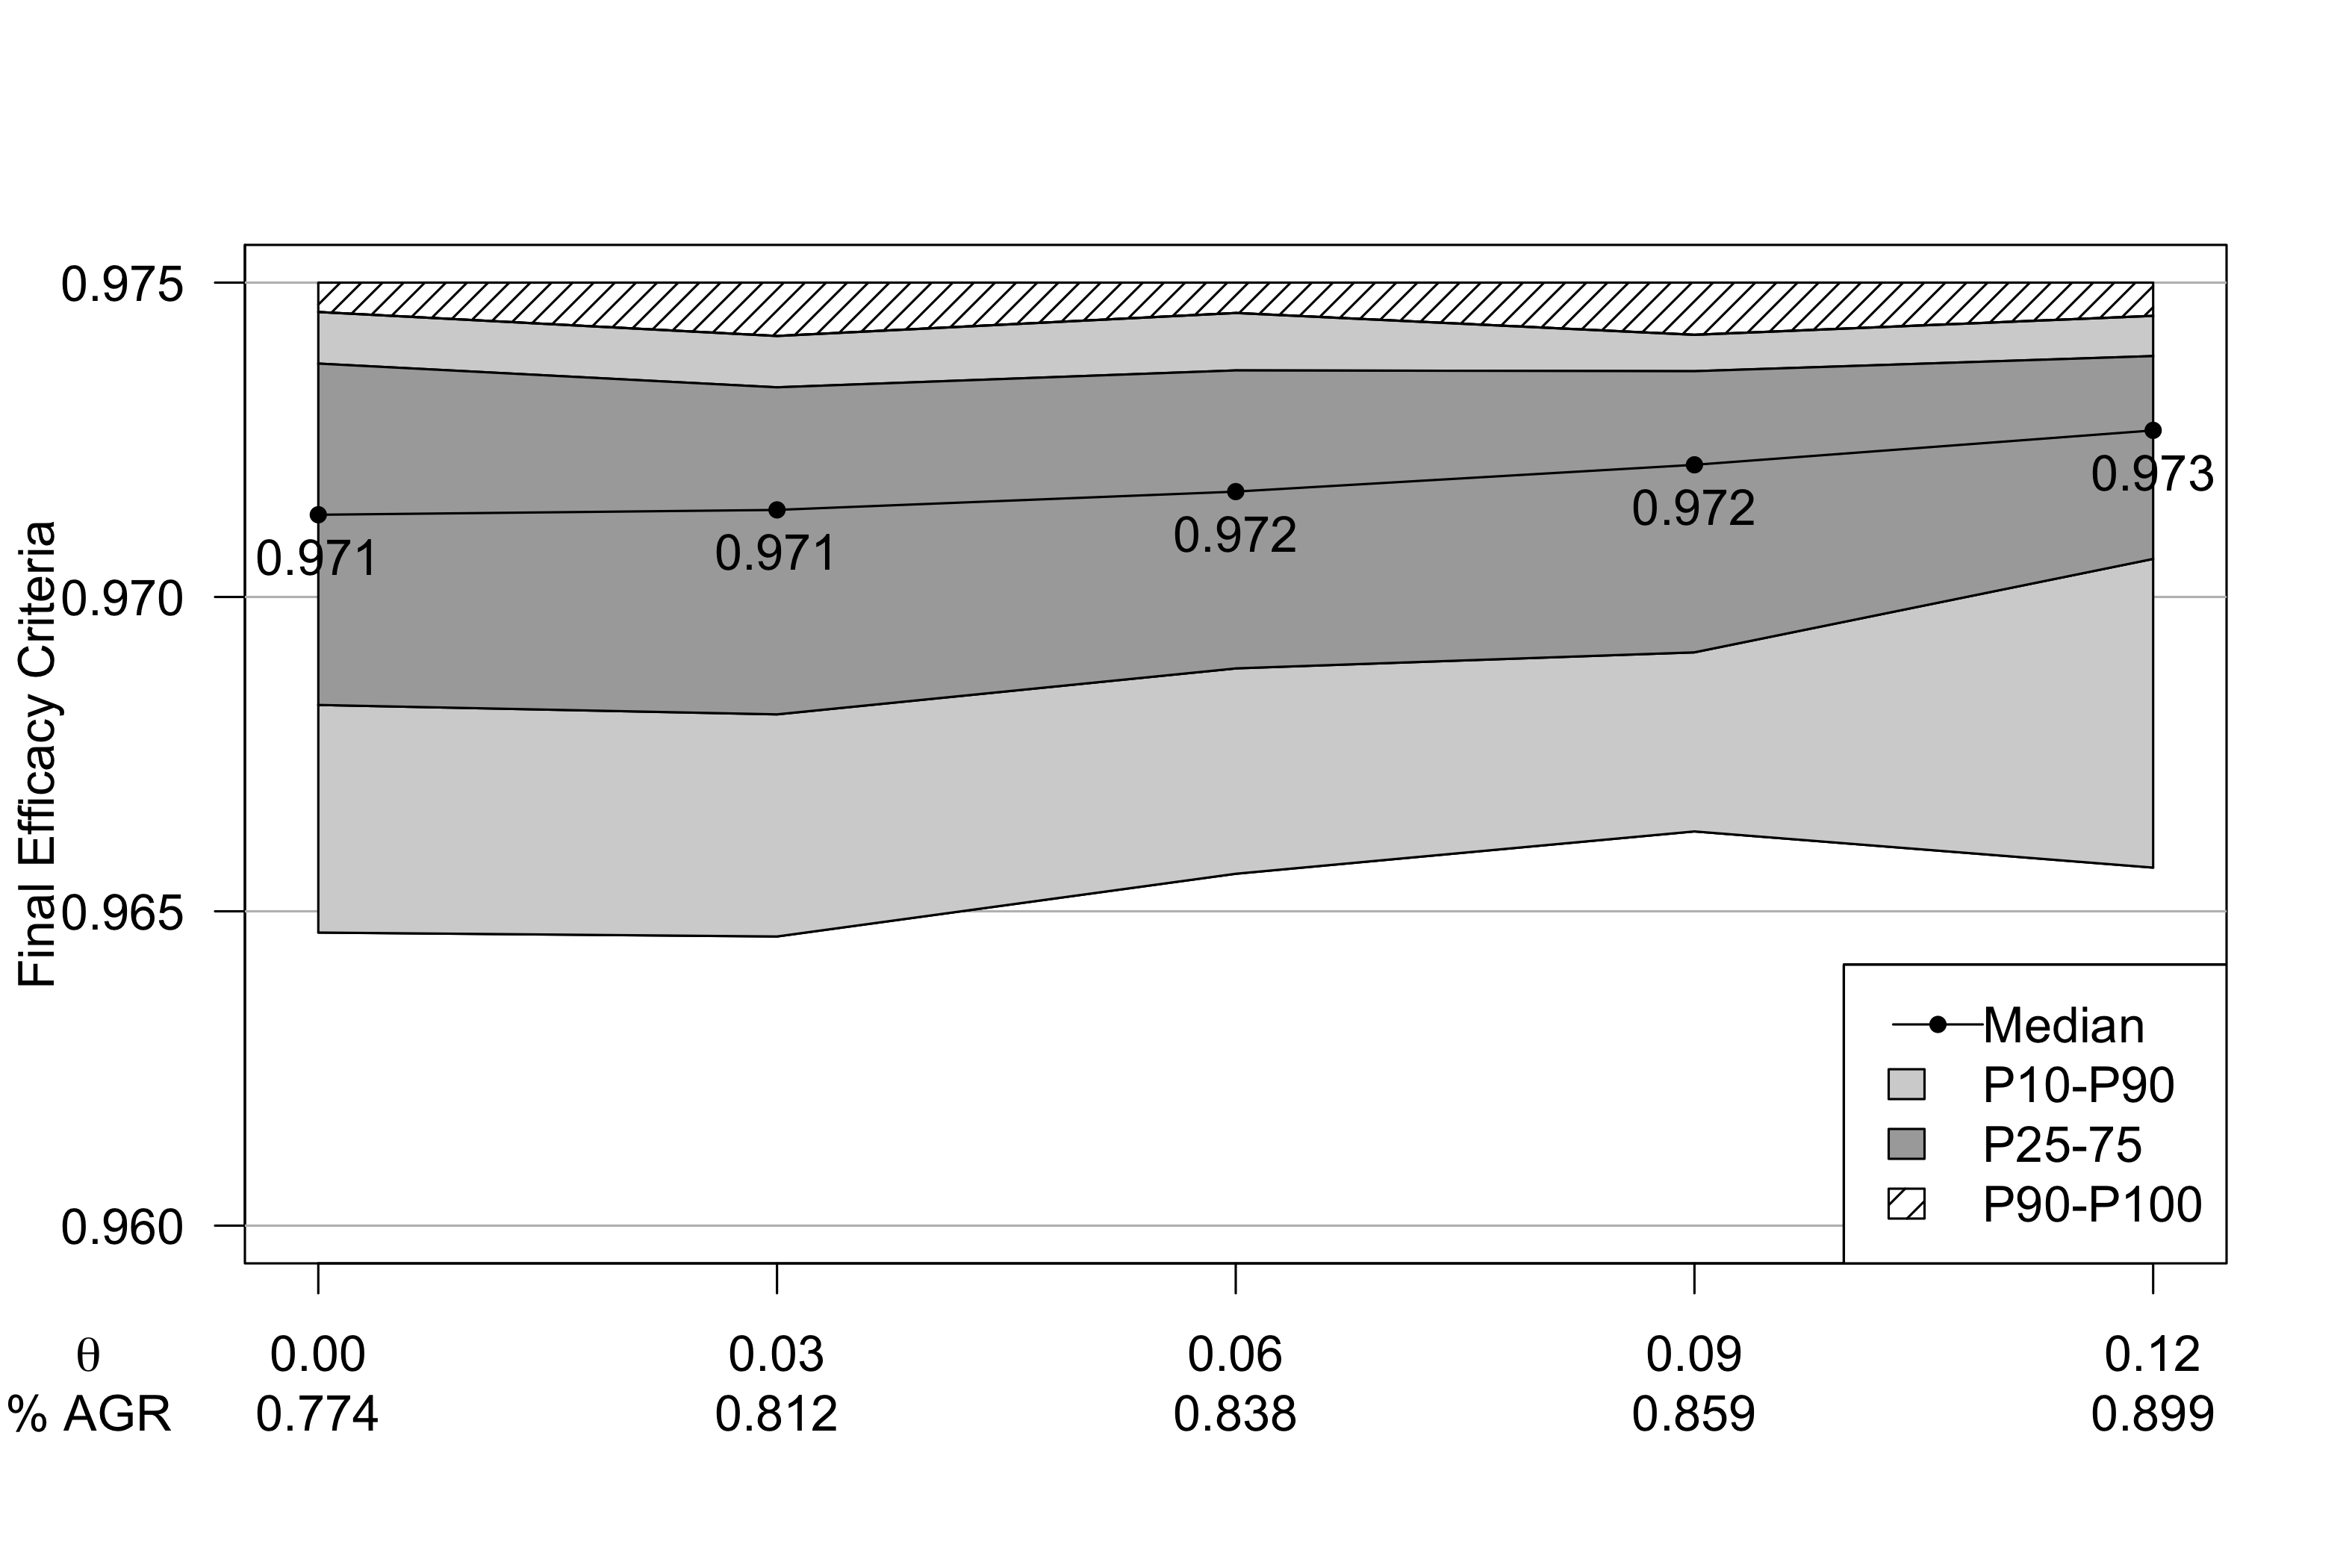
\includegraphics[width=6in]{figure6a.png}
%    \caption{A, Enthusiastic prior mixing weight $\omega$ associated with skeptical prior weight minimum $\delta$ in \eqref{eq:omega} by observed response difference between IP and PC groups, when the PC response rate is fixed at $38\%$ (16/42 responses).}
%\label{fig:ex2varyomega}
% \end{center}
%\end{figure}
%\end{frame}

%\begin{frame}{Operating Characteristics}
%\begin{figure}[htbp]
%\begin{center}
%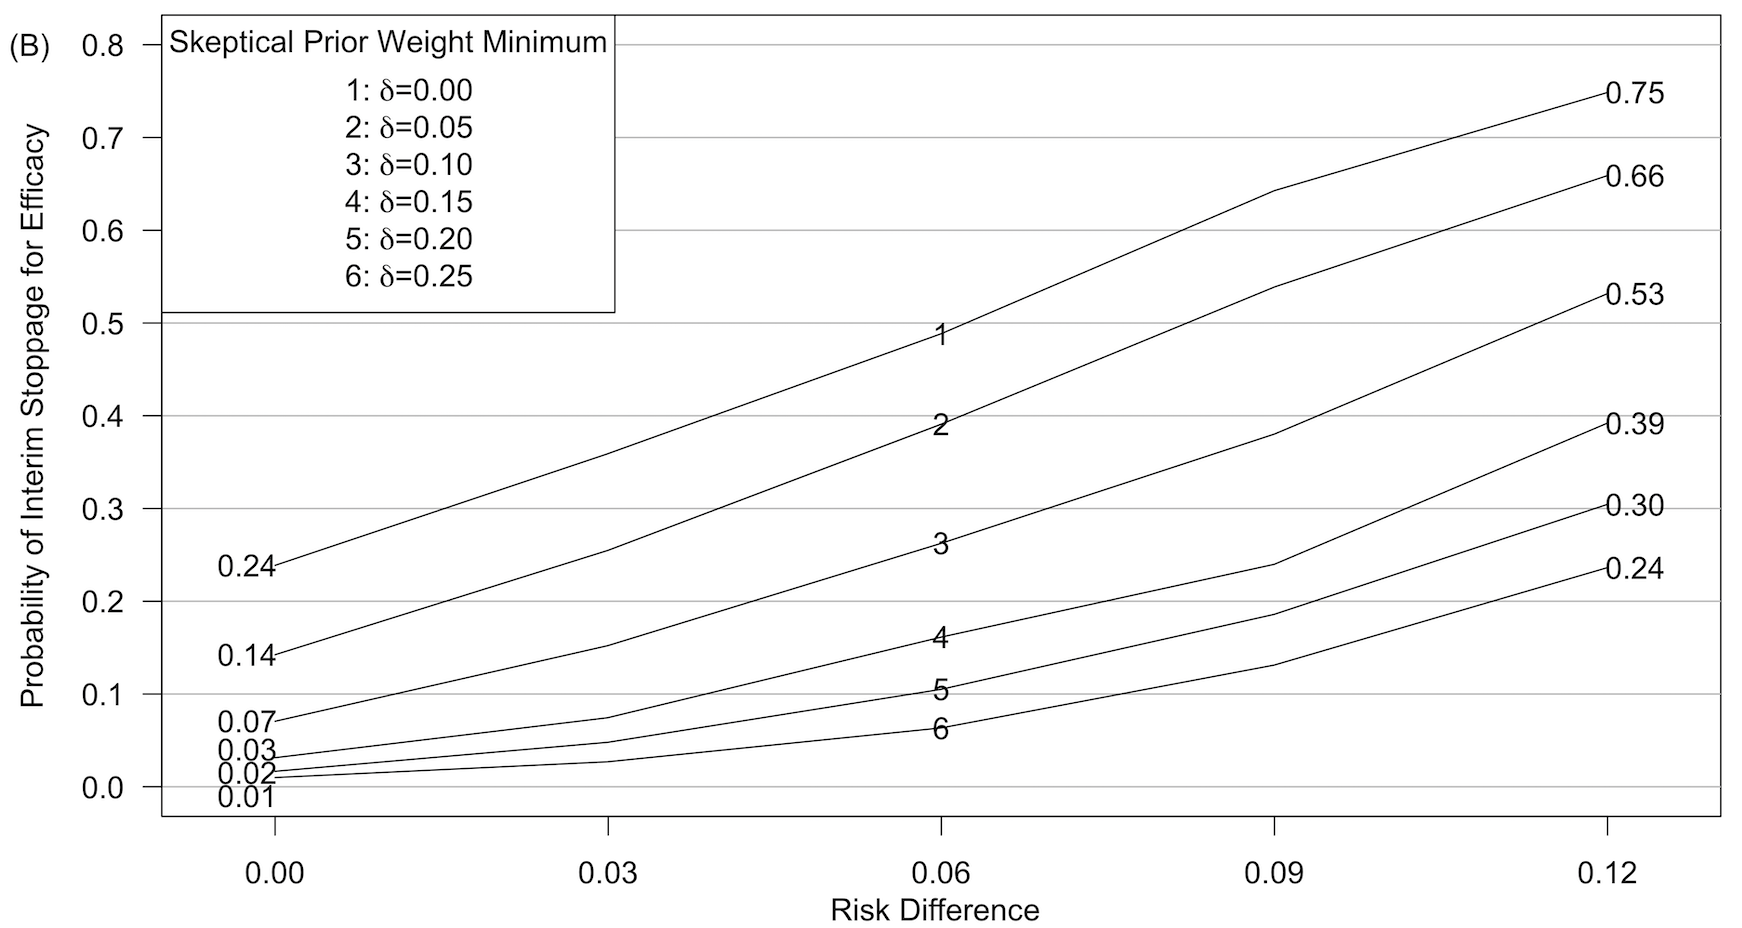
\includegraphics[width=1\textwidth]{./figures/aug12.png}
%%    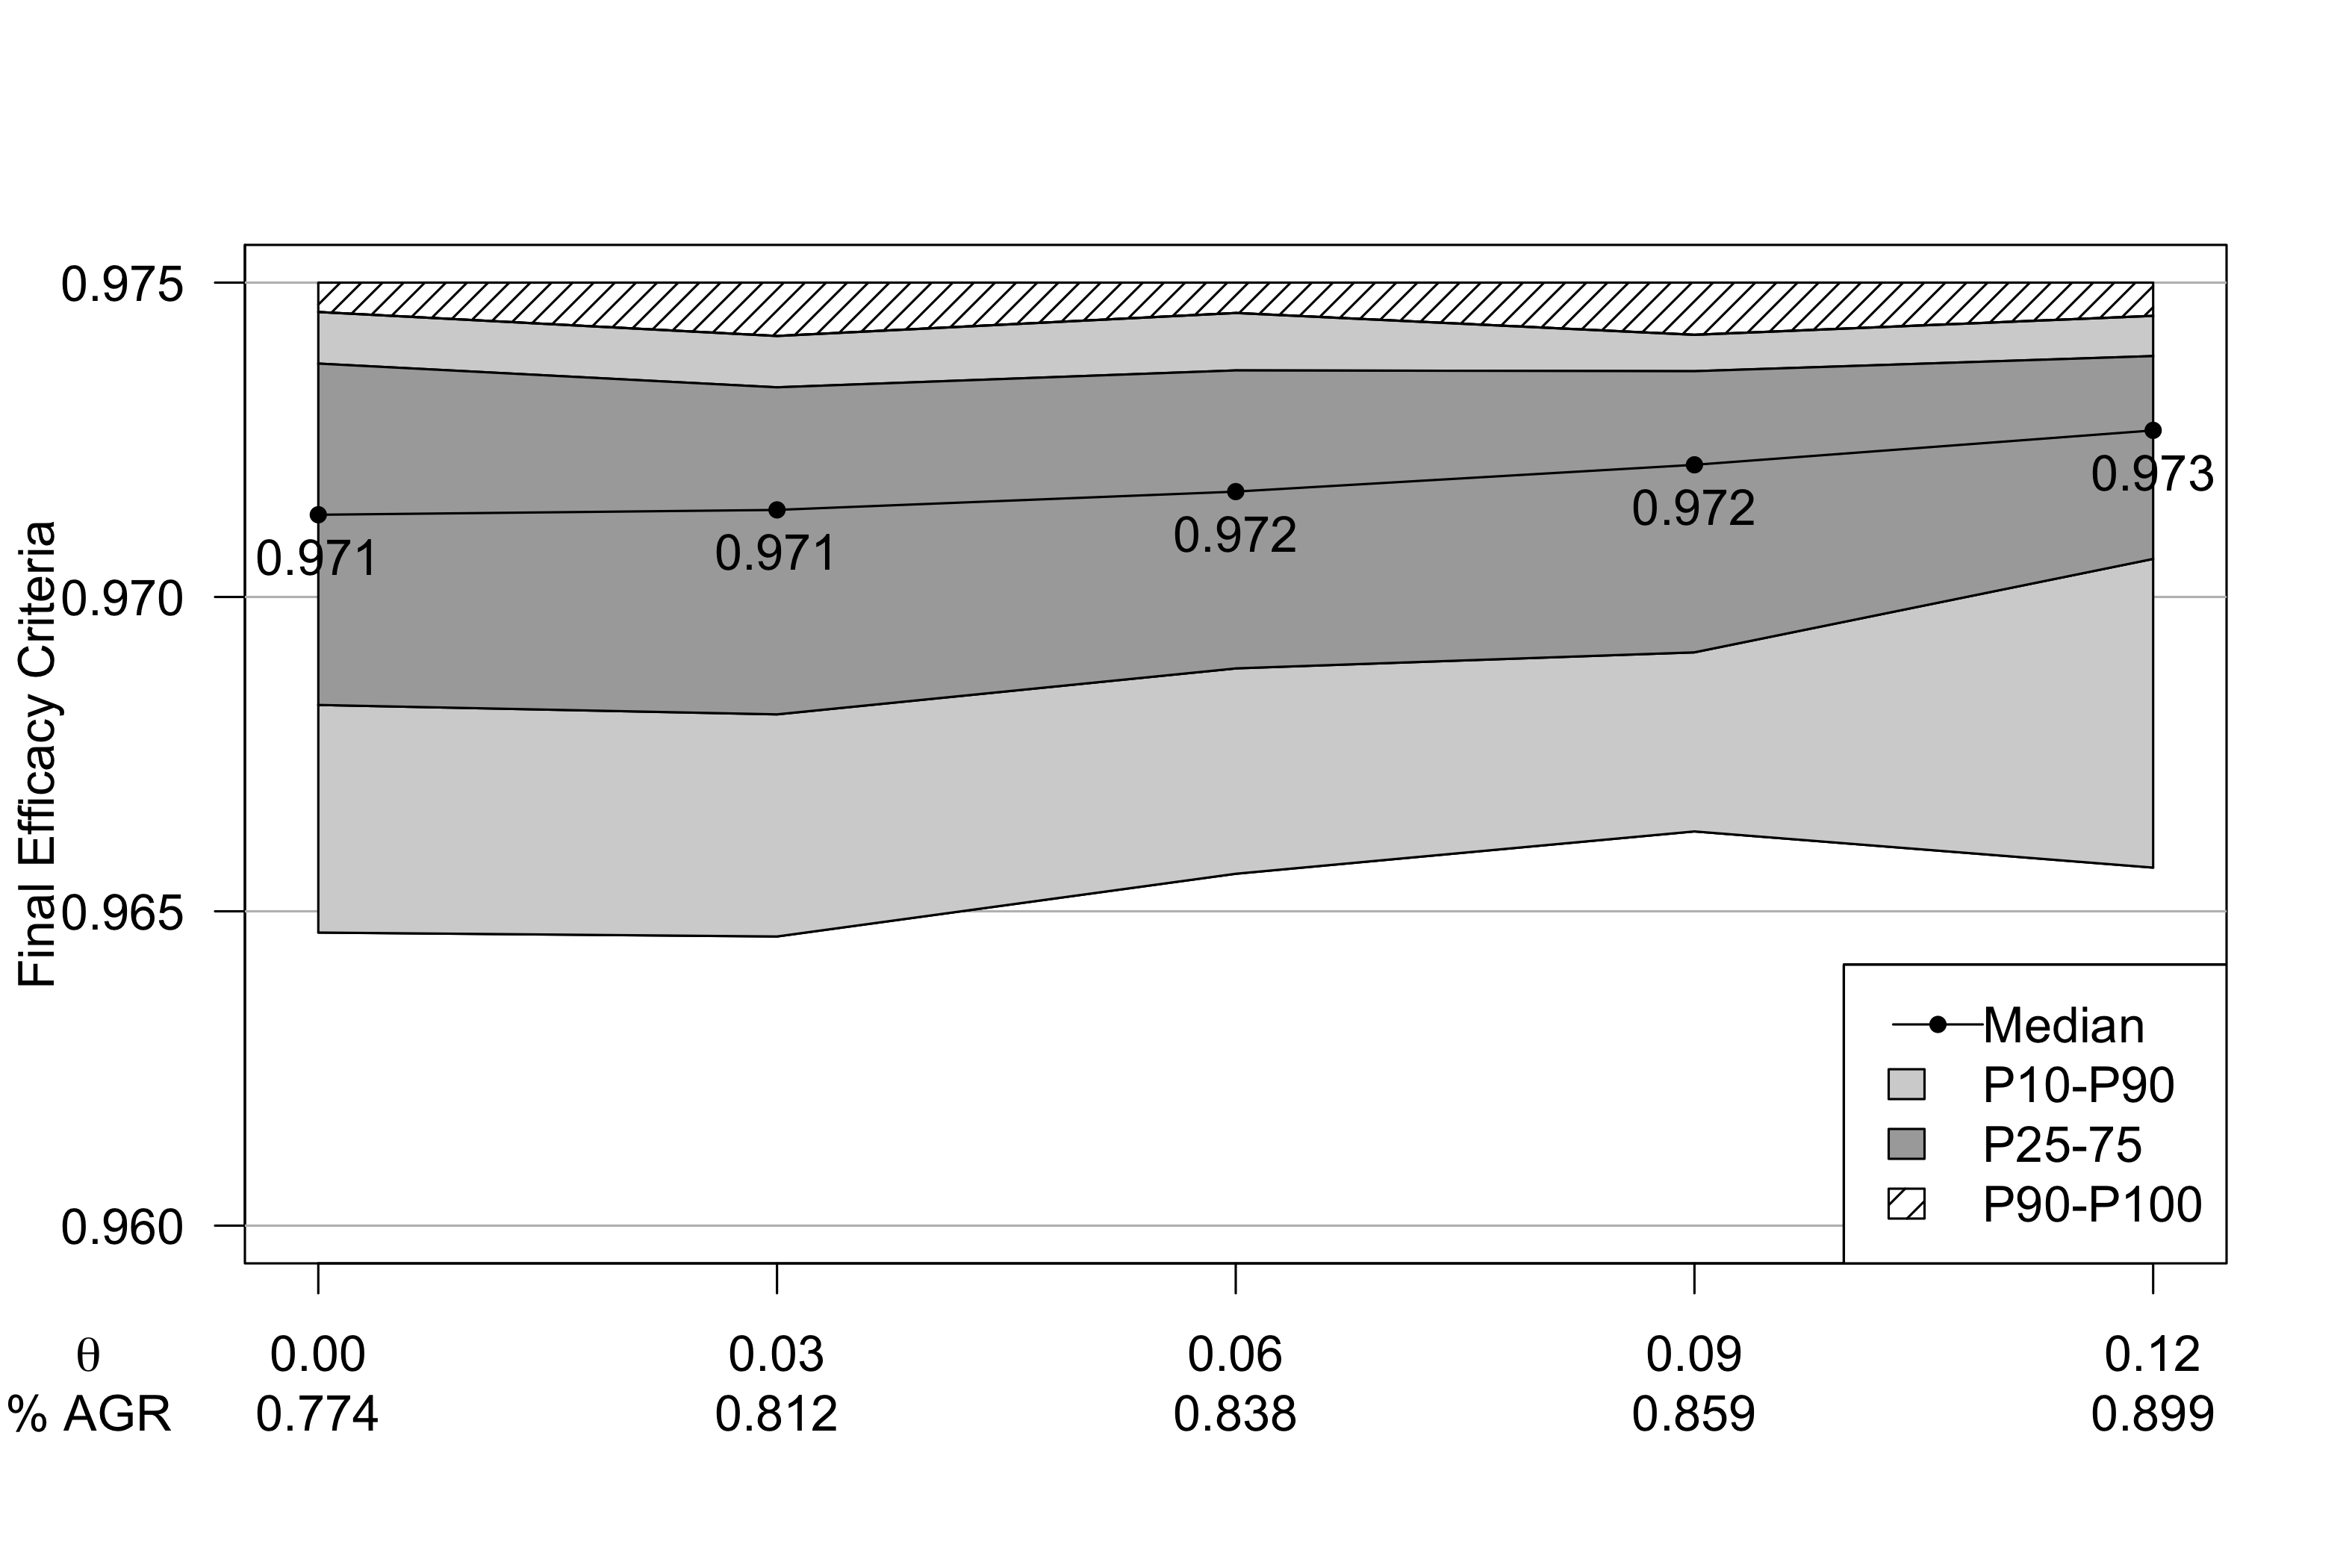
\includegraphics[width=6in]{figure6a.png}
%    \caption{B, Operating characteristics for designs having with skeptical prior weight minimum $\delta$ in \eqref{eq:omega} by true risk difference when the PC response rate generated at $39\%$.}
%\label{fig:ex2varyomega}
% \end{center}
%\end{figure}
%\end{frame}

\begin{frame}{Trial Result}
\begin{itemize}
\item Ultimately, 93 patients were enrolled over approximately 52.5 months (approximately 1 patient enrolled per 17 days).
%
\item Clinical response was observed in 28 of 53 (52.8\%) of patients randomized to belimumab and in 17 of 40 (43.6\%) of patients randomized to placebo (95\% CI [-0.1122, 0.2962]).
\item The data for 1 patient was not available for re-analysis due to a protocol violation.
\item Analyze the data as if it was sequentially monitored after every 2 completed outcomes using the adaptive enthusiastic monitoring prior.
\end{itemize}
\end{frame}

\begin{frame}{Re-analysis of PLUTO trial}
\footnotesize
\begin{table}[htbp]\label{tbl:real-pluto}%
\centering
\caption{Summary characteristics of re-analysis of PLUTO trial. SS = Sample Size, I/F = Interim/Final, $\psi^{(E)}(\mathbf{D}_{\text{obs}})$ = Box's $p$-value using enthusiastic prior, $\omega$ = Enthusiastic mixing weight in adaptive monitoring prior, Efficacy Post Prob = Posterior probability of treatment efficacy.}%
\begin{tabular*}{300pt}{@{\extracolsep\fill}ccccc@{\extracolsep\fill}}%
\toprule
SS (I/F)			&	$\psi^{(E)}(\mathbf{D}_{\text{obs}})$ (I/F)			&	$\omega$ (I/F)			&	Efficacy Post Prob (I/F)			\\
\midrule
62	/	90	&	0.914	/	0.965	&	0.914	/	0.965	&	0.980	/	0.979	\\
\bottomrule
\end{tabular*}
\end{table}
\end{frame}

\begin{frame}{Box's $P$-value Using Enthusiastic Prior $\psi^{(E)}(\mathbf{D}_{\text{obs}})$ }
\begin{figure}[htbp]
\begin{center}
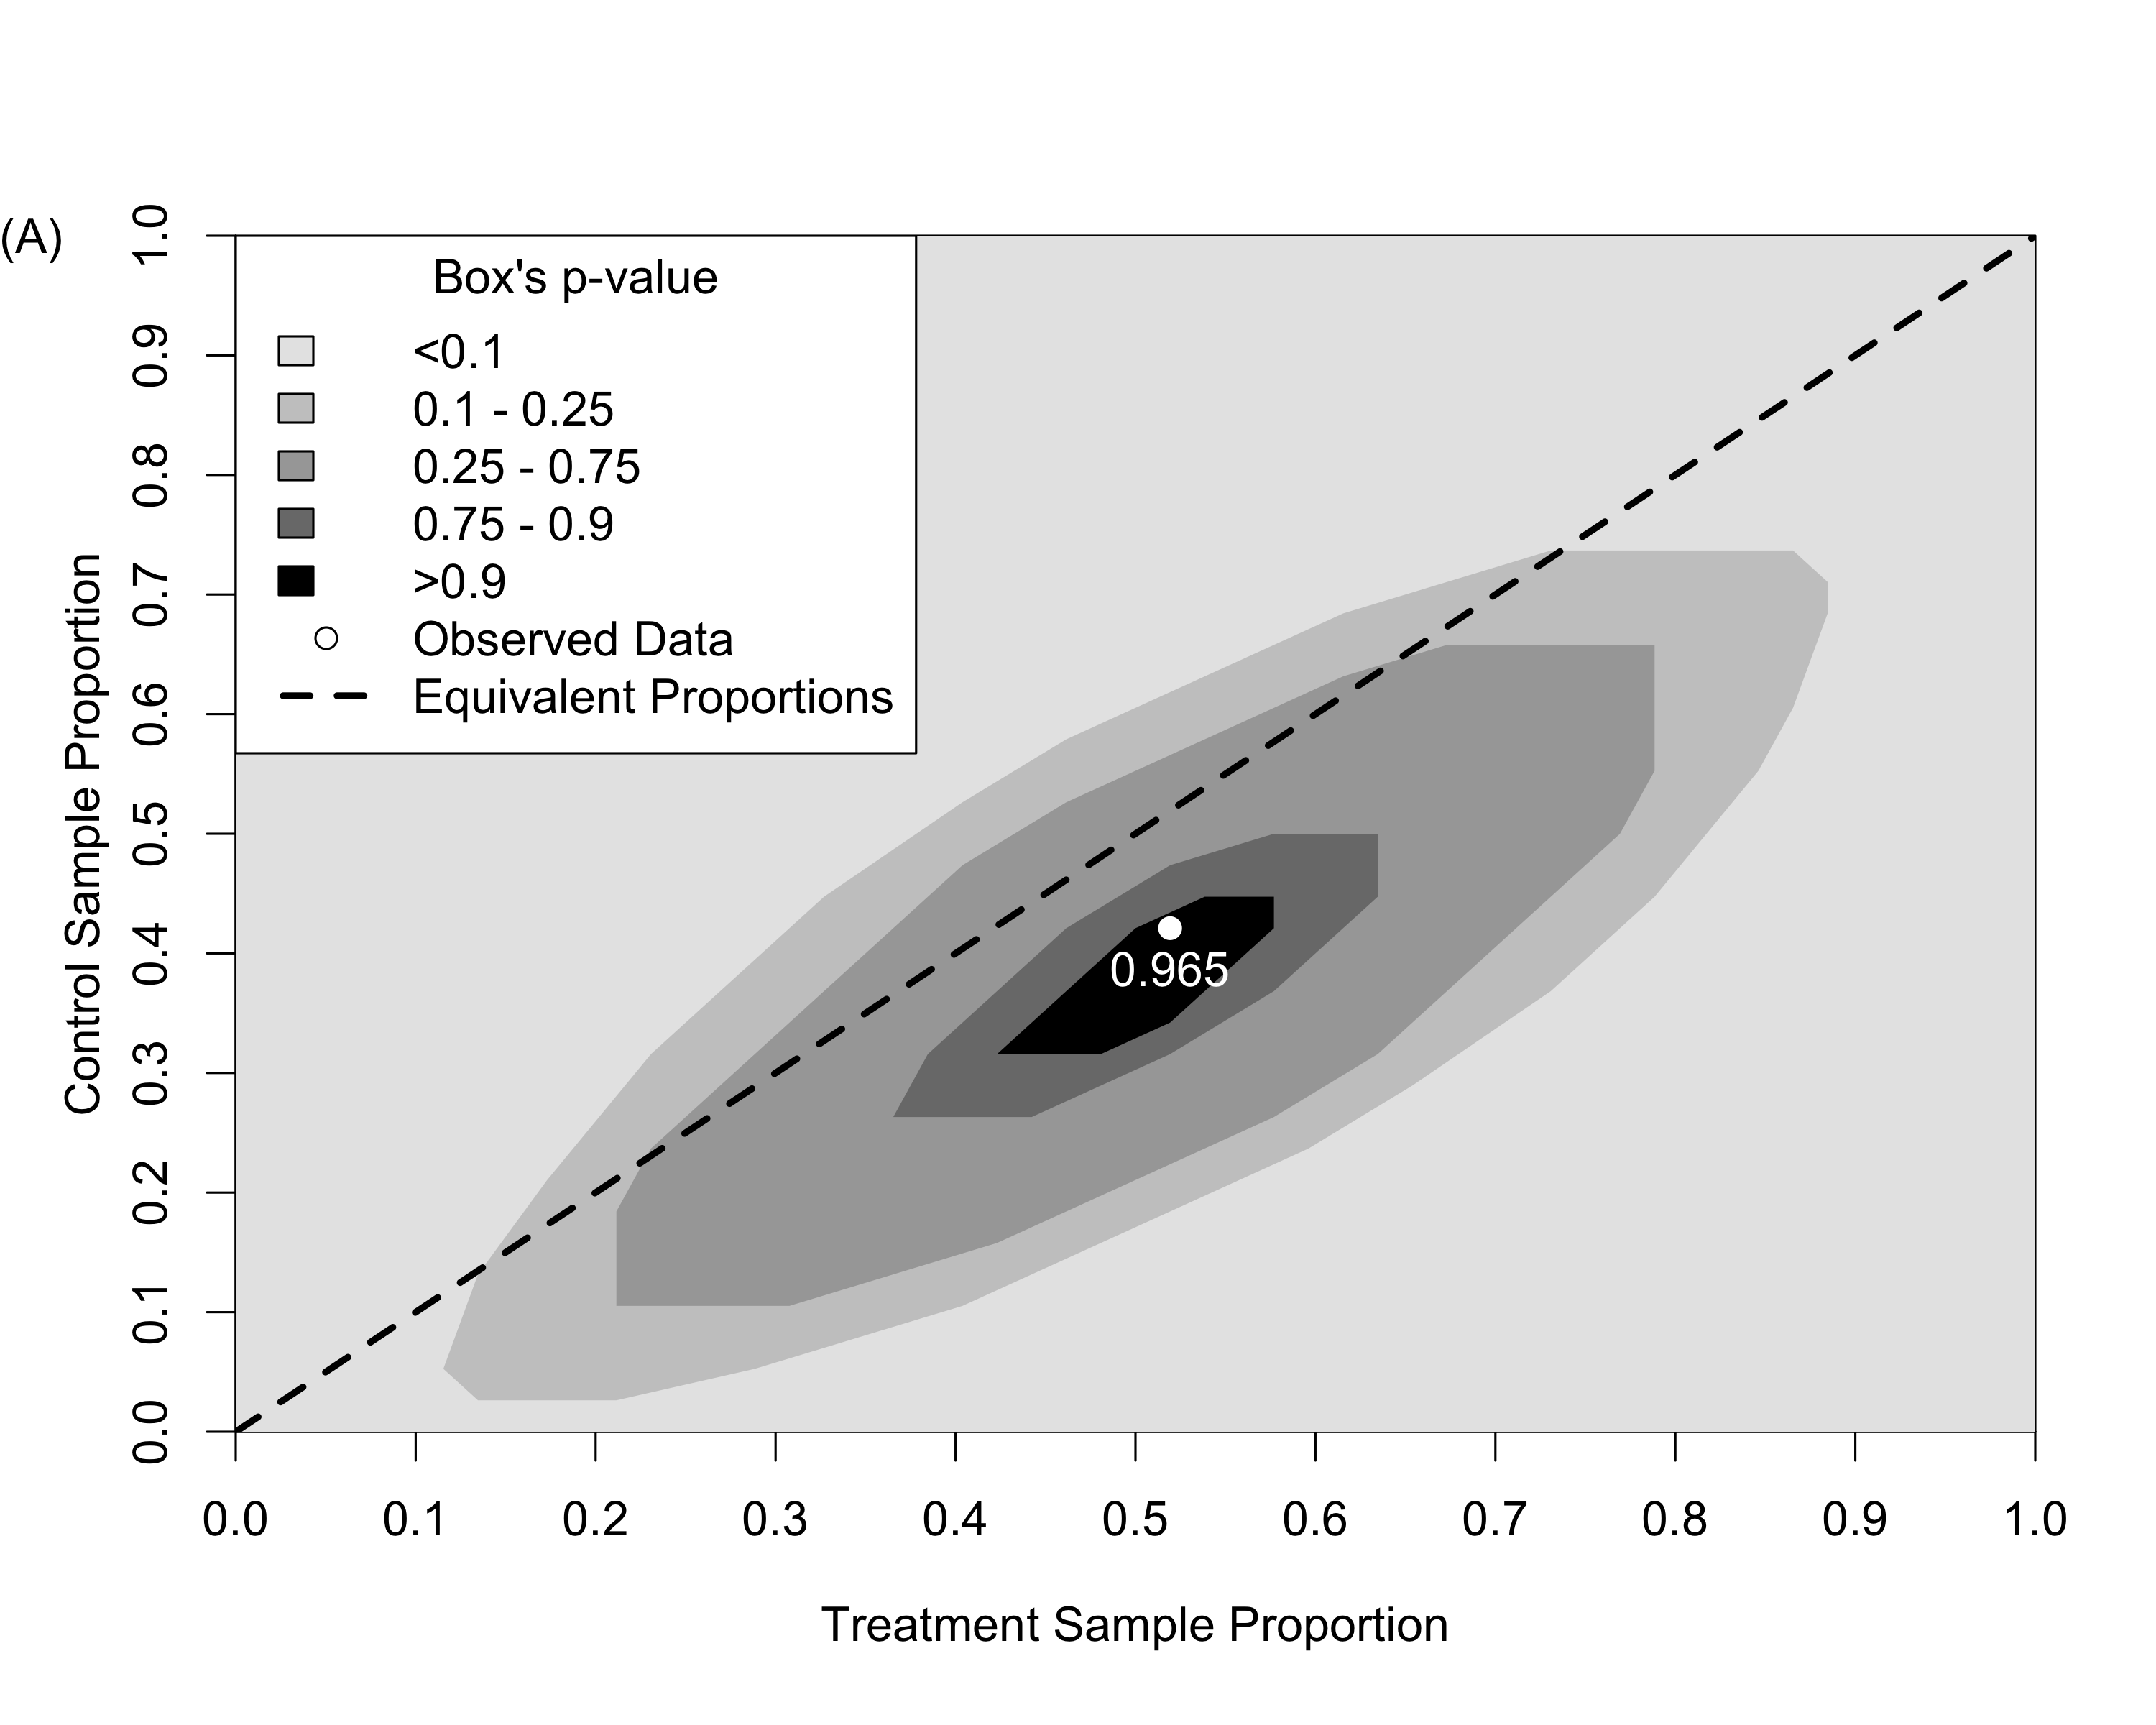
\includegraphics[width=0.7\textwidth]{./figures/2dbayesp.png}
    \caption{A, Box's p-value by control and treatment sample proportions at the final analysis with 90 subjects when $\delta=0$ is used \eqref{eq:omega} for the adaptive monitoring prior.}
\label{fig:2dheatmaps}
 \end{center}
\end{figure}
\end{frame}

\begin{frame}{Posterior Probability of Treatment Efficacy}
\begin{figure}[htbp]
\begin{center}
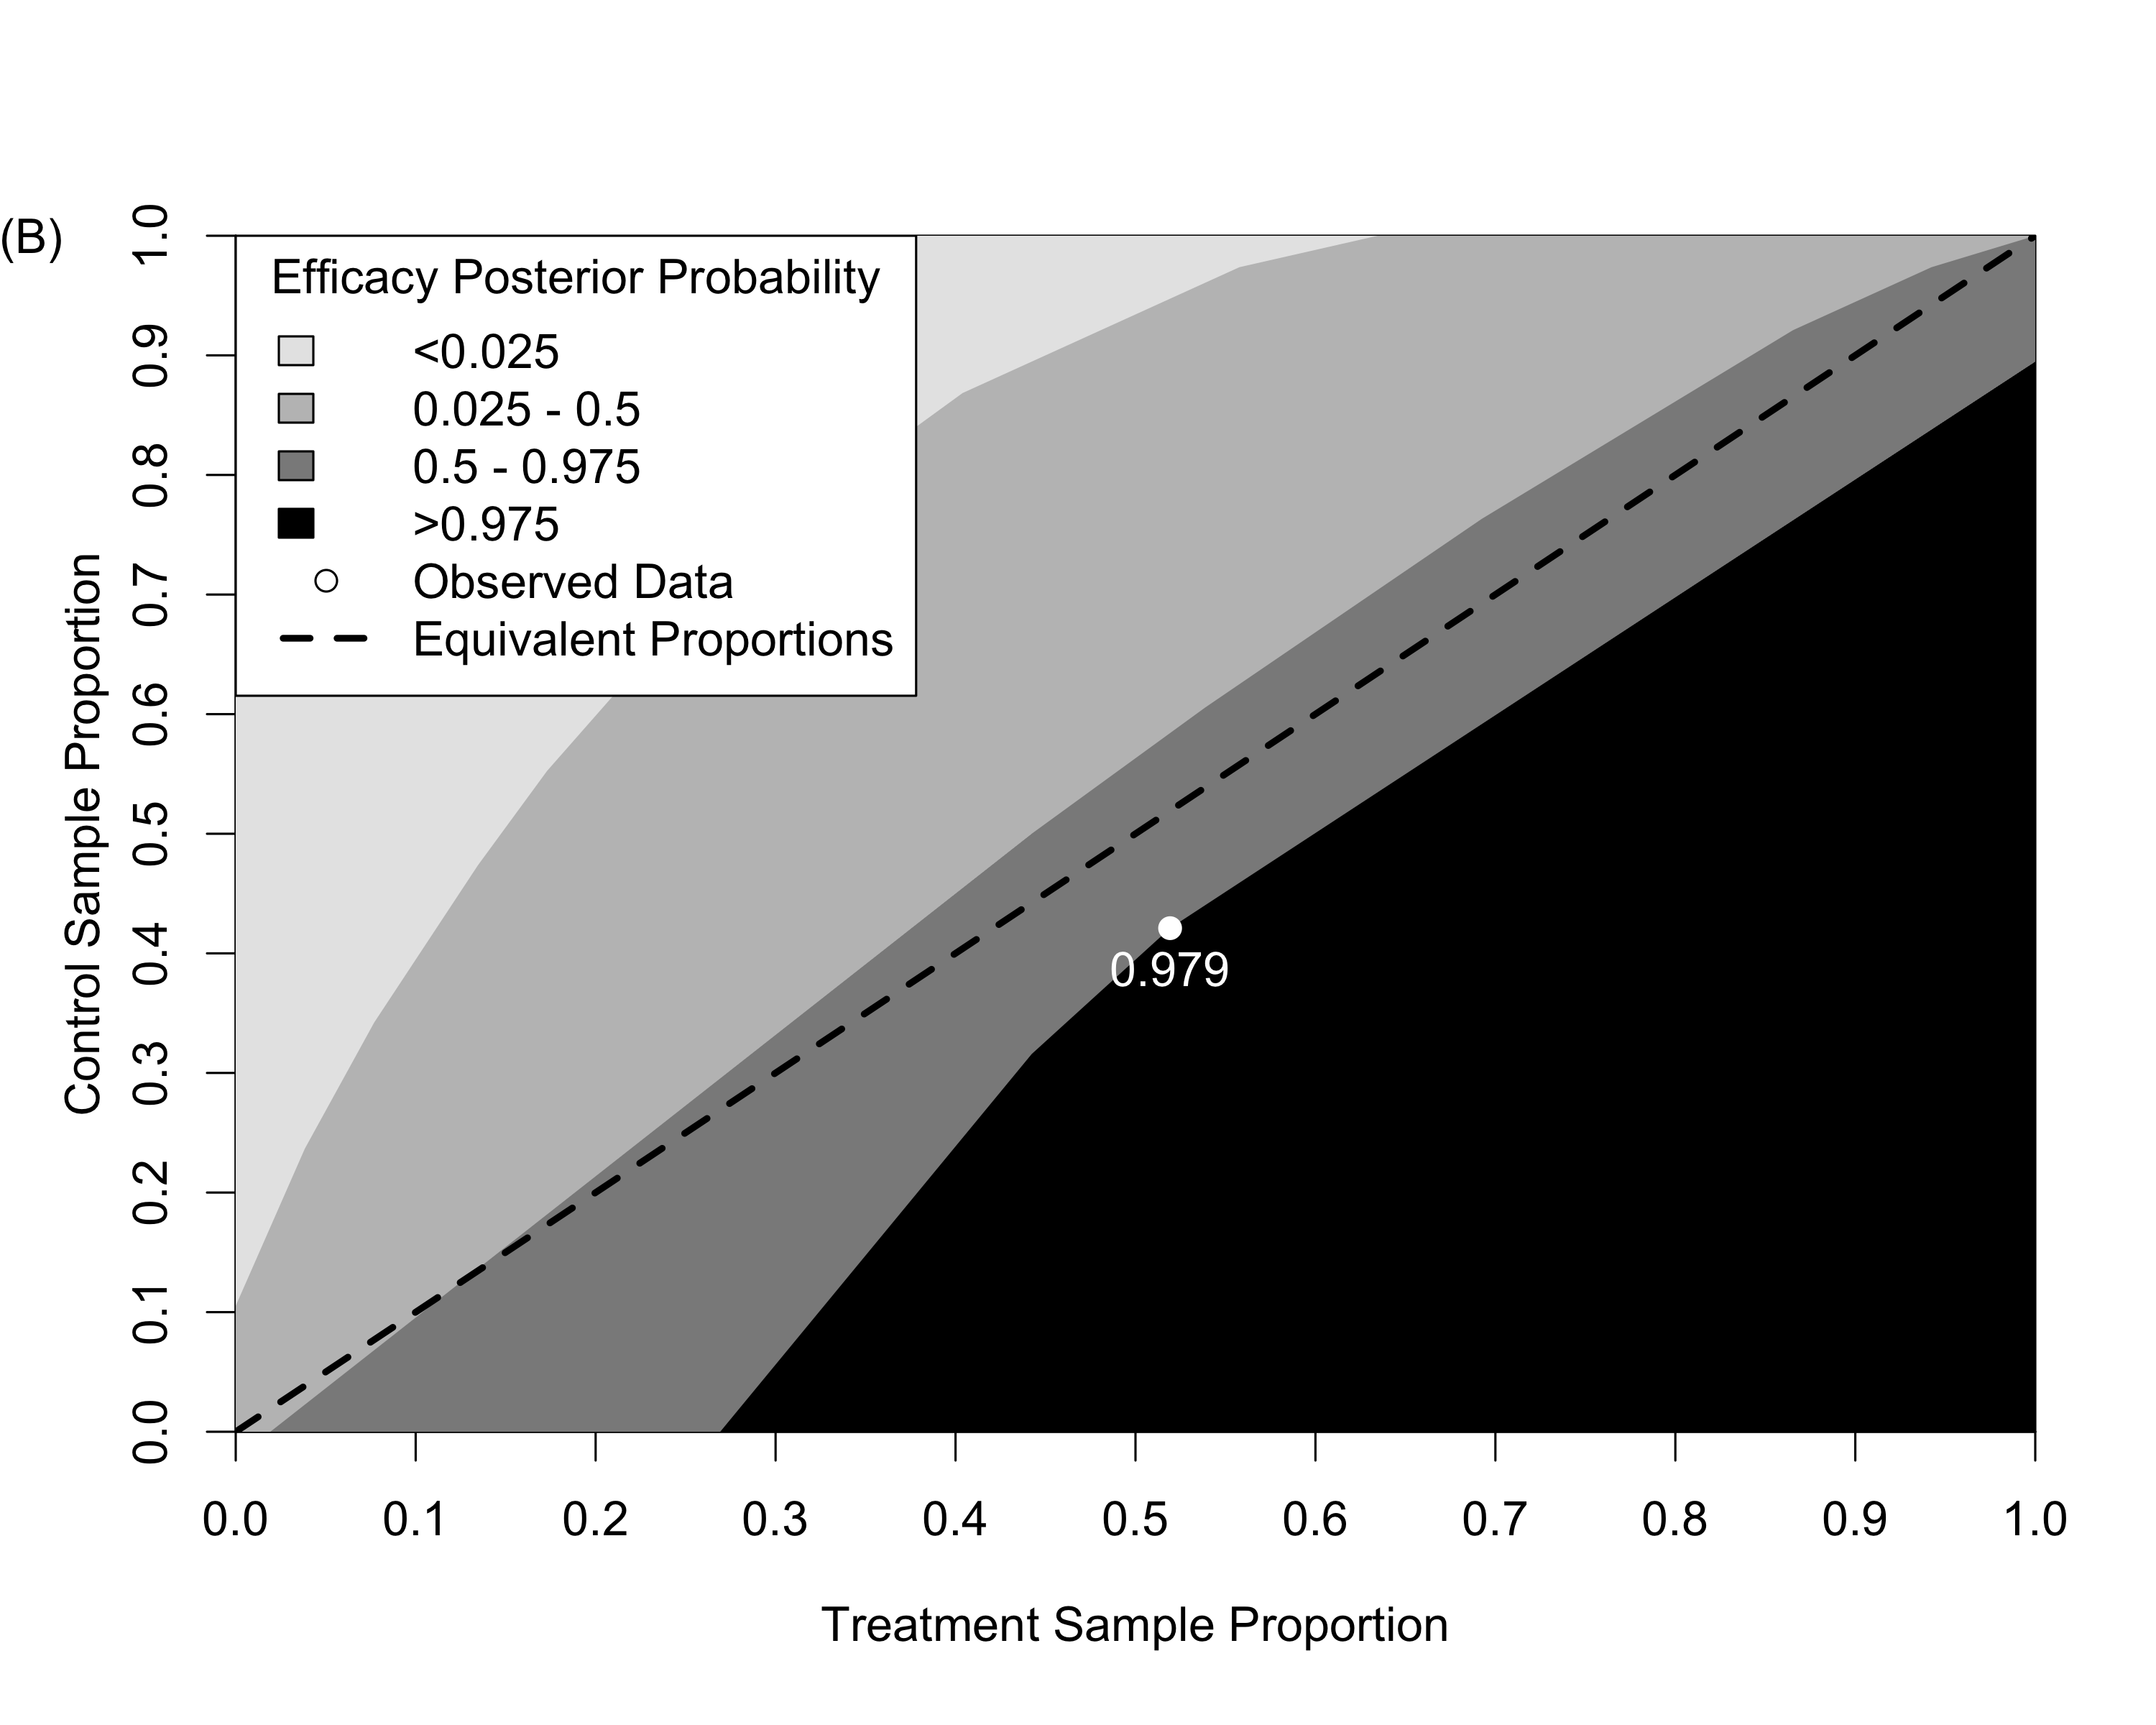
\includegraphics[width=0.7\textwidth]{./figures/2dpostp.png}
    \caption{B, Posterior probability of efficacy by control and treatment sample proportions.}
\label{fig:2dheatmaps}
 \end{center}
\end{figure}
\end{frame}





%
%\begin{frame}{Discussion}
%\begin{itemize}
%\item 
%\end{itemize}
%\end{frame}

\begin{frame}{References}
%\bibliographystyle{agsm} 
\bibliographystyle{natbib}
\bibliography{./References}	
%\bibliography{FinalDissertationReferences.bib}
\end{frame}

\end{document}